\chapter{Discussion and Comparison} \label{discussion-and-comparison}

At first glance, the results in \cref{results} look promising. The problematic obstacles in \cref{traditional-obstacle-sensors} that provided the motivation for this work (windows and chairlegs) appear on the maps in \cref{fig:pres3,fig:pres4}. The following section takes a detailed look at some of the qualities outlined in \cref{evaluation} by analyzing some effects which are visible in the radar scans.

\section{Discussion}

\subsection{Reflection directionality} \label{reflection-directionality}

Many objects only become visible when their surface is oriented
perpendicularly to the incident radar waves, so that enough scattered EM
energy makes its way back to the sensor. This is very visible in the
Underground scan, where a glass wall is detected as the robot passes it,
but not while the robot sees it at an angle.

In the Torture Chamber scan, the same effect is visible for chair legs,
especially for the chair at the scene center. The legs appear in clear
form as soon as the radar sees them from a point that is orthogonal
to the office chair legs.

This means that in an online mapping process, obstacles might appear earlier or later, depending on their orientation towards the radar position. The effect is expected and was decribed in \cref{limitations}.


\subsection{Material-dependent echo strength} \label{material-dependent-echo-strength}

Some materials, like metal, are better at reflecting radar
waves than others, like Styrofoam. Due to their electrical conductivity, metal objects cause particularly strong echos which are visible from a higher distance. This can be observed in the hallway scans (e.g.~Orbit, Public Restroom, Queue,
Racetrack, Sauna, Underground), where the metal frames of doors and
glass walls stand out in the scan.

\subsection{Doppler vs Direction of Arrival data quality} \label{doppler-vs-direction-of-arrival-data-quality}

In forward-facing geometry (scans D--T), the DOA is necessary to resolve
the sign of a target's reprojection angle. This works fairly well, for
example at the start of Sauna (see \cref{fig:sauna_doa}), the closer target
passes on the right (more pink), while the other targets stay to the
left side of the robot (more green).

\begin{figure}[htbp]
    \centering
    \begin{subfigure}[b]{0.45\textwidth}
        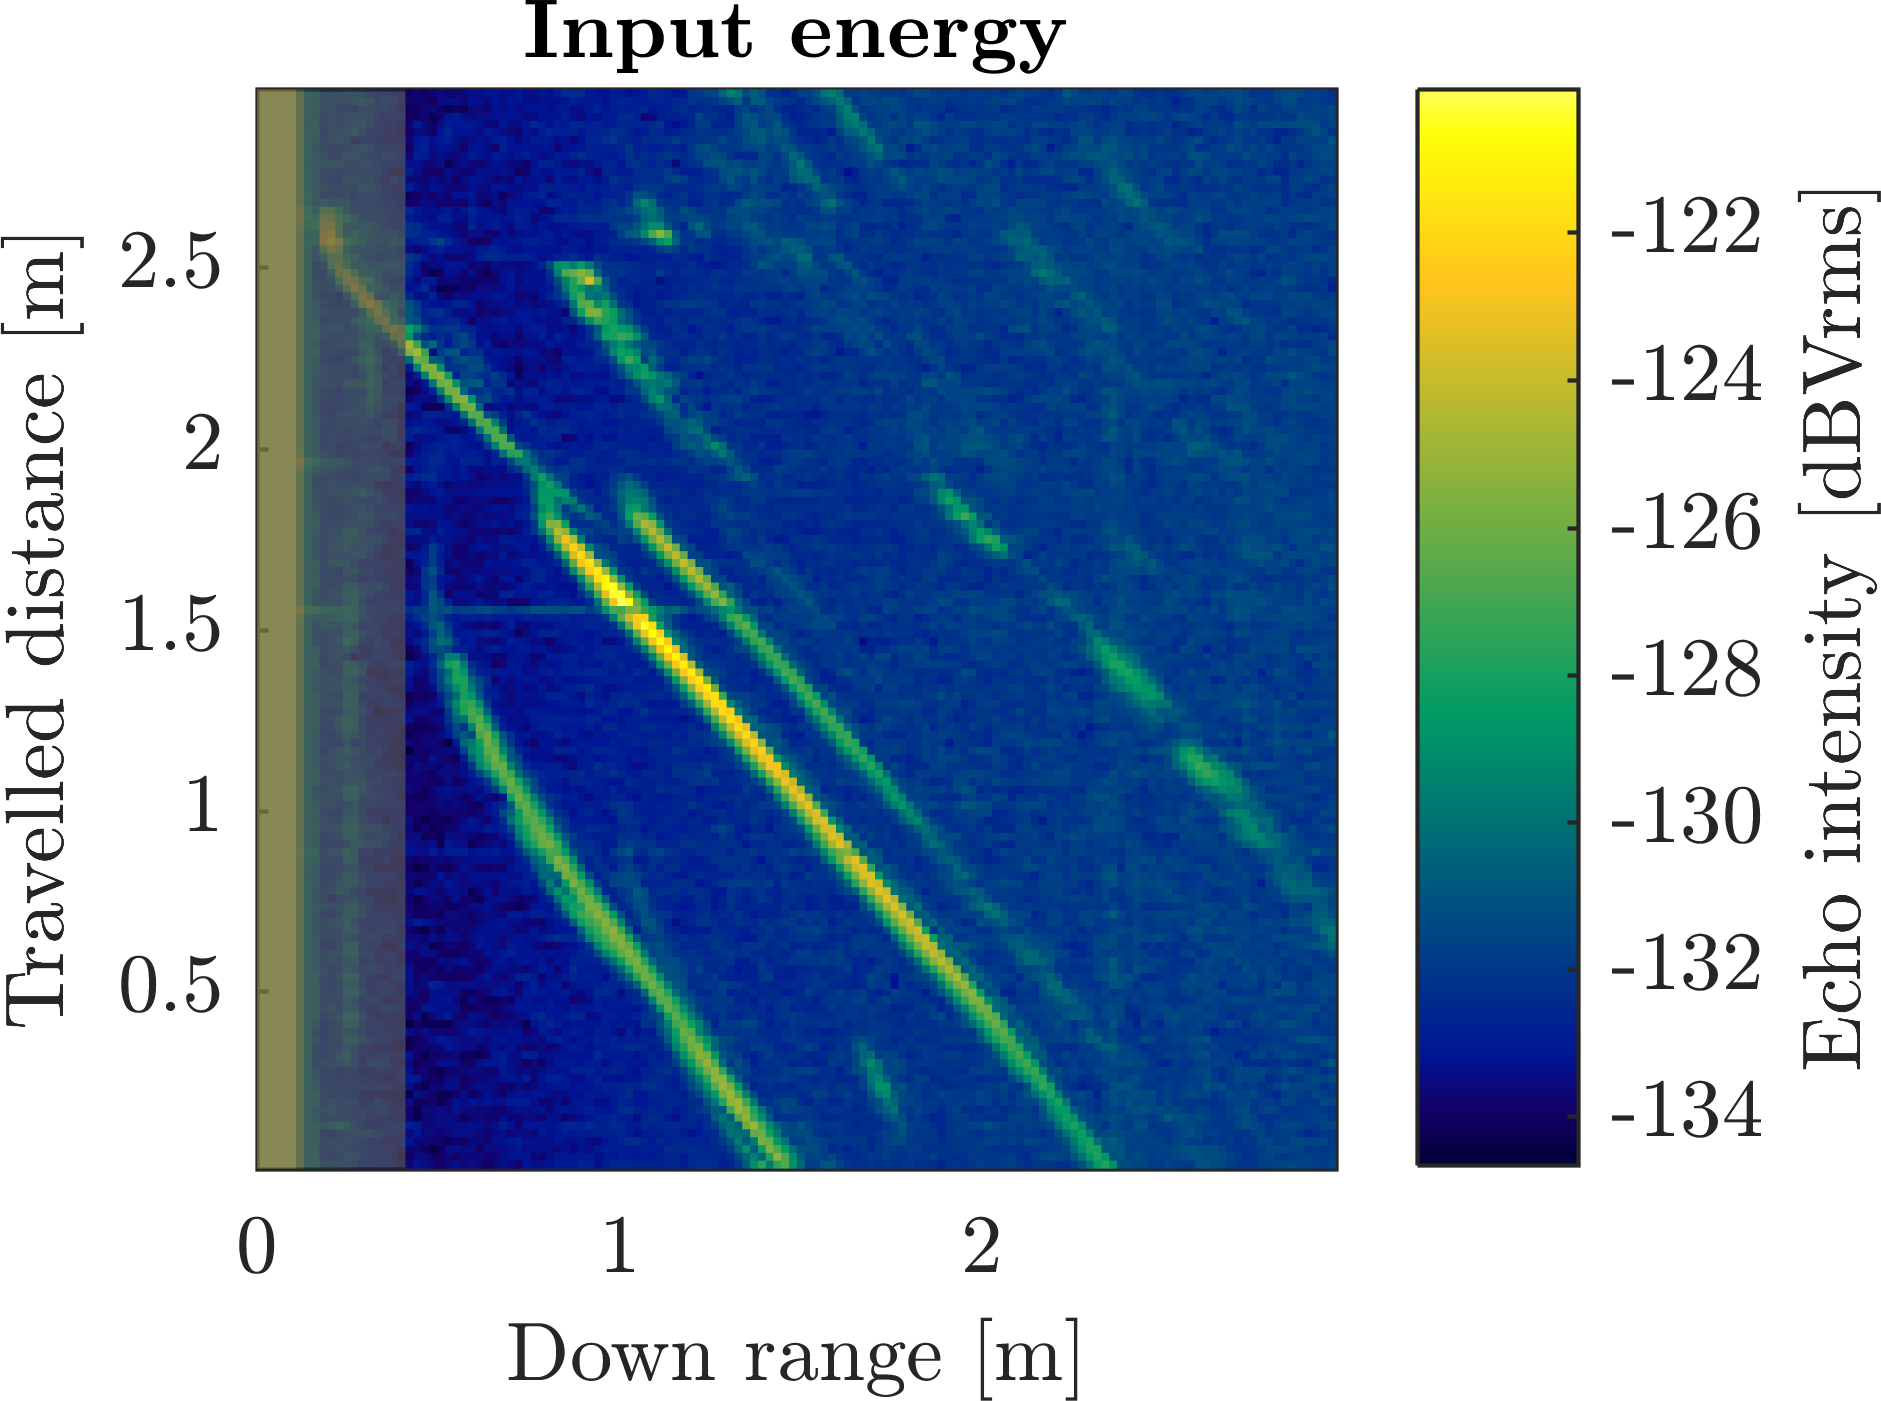
\includegraphics[width=\linewidth]{figures/fig_doa_sign_input.png}
        \caption{\label{fig:sauna_input}Echo intensity}
    \end{subfigure}%
    \hfill%
    \begin{subfigure}[b]{0.45\textwidth}
        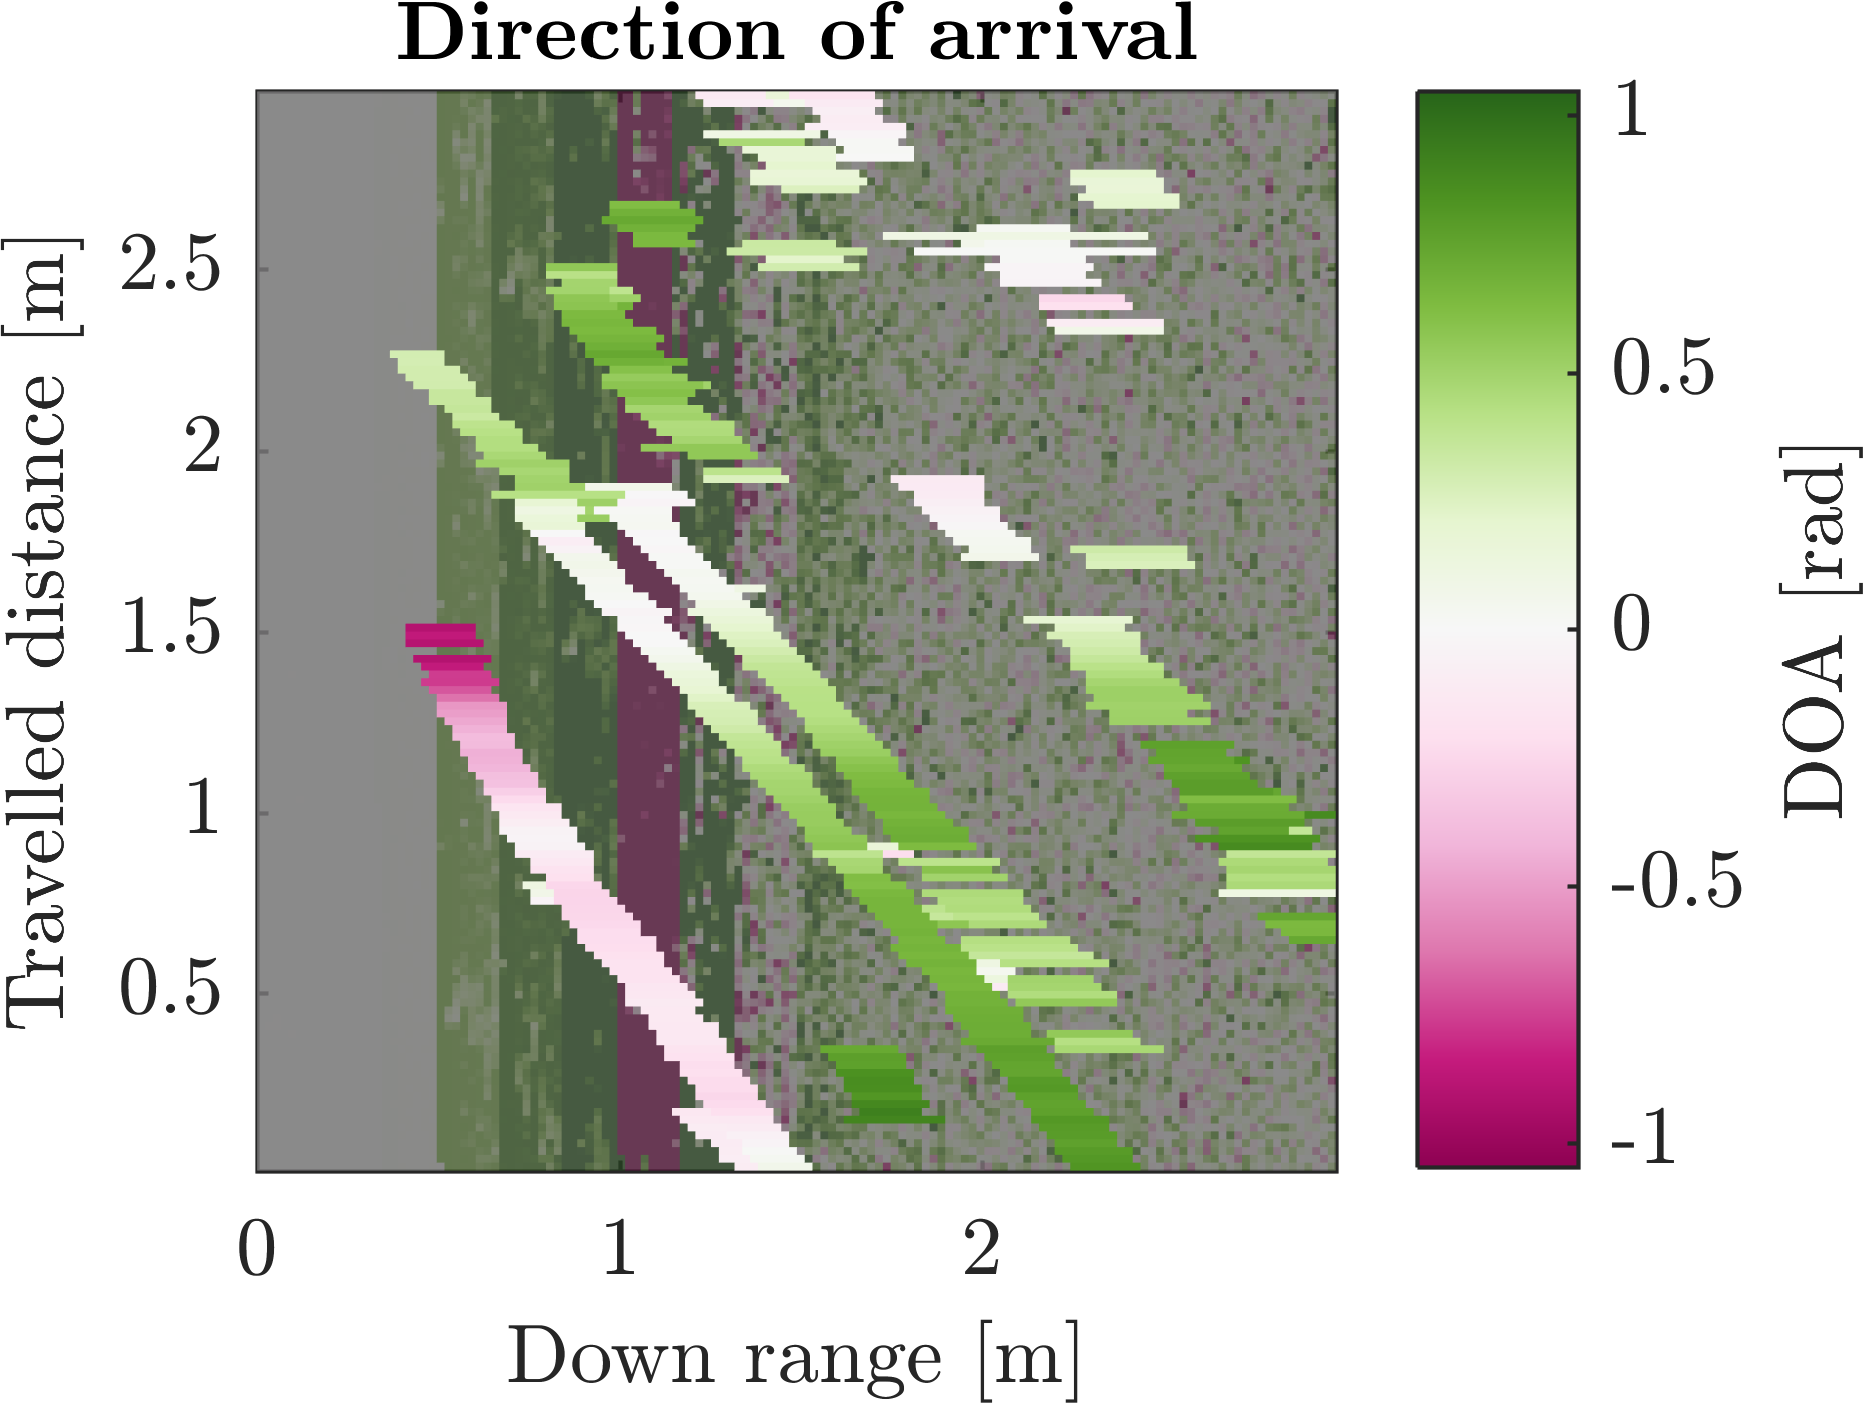
\includegraphics[width=\linewidth]{figures/fig_doa_sign_doa.png}
        \caption{\label{fig:sauna_doa}Direction of arrival estimation}
    \end{subfigure}
    \caption{Range profile and DOA of Sauna scan.}
    \label{fig:sauna}
\end{figure}

In fact, for the side-facing case, the smoothed DOA data also turned out
to be very good (angular error is usually less than \ang{10}). In combination with a sensor fusion approach, it might even be used to calculate a more precise
reprojection angle.

Both the forward- and side-facing geometry DOA data is sensitive to the rotation of the radar's antenna with respect to the radar motion path. When the DOA sign is used for angle ambiguity resolution, errors can thus appear at angles near \ang{0}. The effect does not have a drastic effect on map quality though, because angle sign errors do produce phantom targets at wrong map locations at large angles (e.g. \ang{90}), but still yield similar positions at small angles (i.e. mostly straight ahead).

\subsection{Multipath effects}\label{multipath-effects}

Multipath effects are a well-known problem in ground-based radar
applications \cite{Adams2012}. In situations where multi-path effects
are likely, there is a higher possibility that multiple versions of a
target's echo are visible, which can lead to detection of incorrect
angle and ranges. Luckily, in the recorded data almost no multipath
effects are obvious. The only scan that shows some effects is the
Torture Chamber. There, it seems like the radar waves bounce around a
bit in the area with highly reflective metal cabinets under the desk around (\SI{2}{m},\SI{2}{m}). The effect is that some targets are detected behind the wall behind the desk. It can be expected to be less noticeable in residential environments, which contain fewer (if any) metal corners.

\subsection{Object penetration}\label{object-penetration}

Some objects are penetrated by the radar waves. For example, in the
Attic and Basement scans, both the front and the back wall of a
plastic bottle can be seen. However, the plastic bottle was relatively
close to the sensor. On the other hand, in the scans with glass walls in
them (P,Q,R,S,U), no significant radar echo is picked up from the
(metal) chair legs behind the glass wall. This is because a typical
glass pane attenuates the \SI{60}{GHz} signal by about \SI{5.5}{dB} \cite{Lu2014}. In
effect, a radar sensor with higher transmission power might be able to
see through walls, but in the conducted experiments radar echos were to
faint to be picked up after the first bigger object (like a wall).
This is OK, because obstacles that are behind walls don't pose an immediate threat that needs to be circumnavigated. Through-wall visibility would mostly be interesting in slam applications that use the mapped objects for localization.

\subsection{Negative obstacles}\label{negative-obstacles}

\begin{figure}[htbp]
% 0.95 * 2832*2268/2124 / (2832*2268/2124 + 3024) = 0.475
% 0.95 * 3024 / (2832*2268/2124 + 3024) = 0.475
    \centering
    \begin{subfigure}[t]{.475\textwidth}
        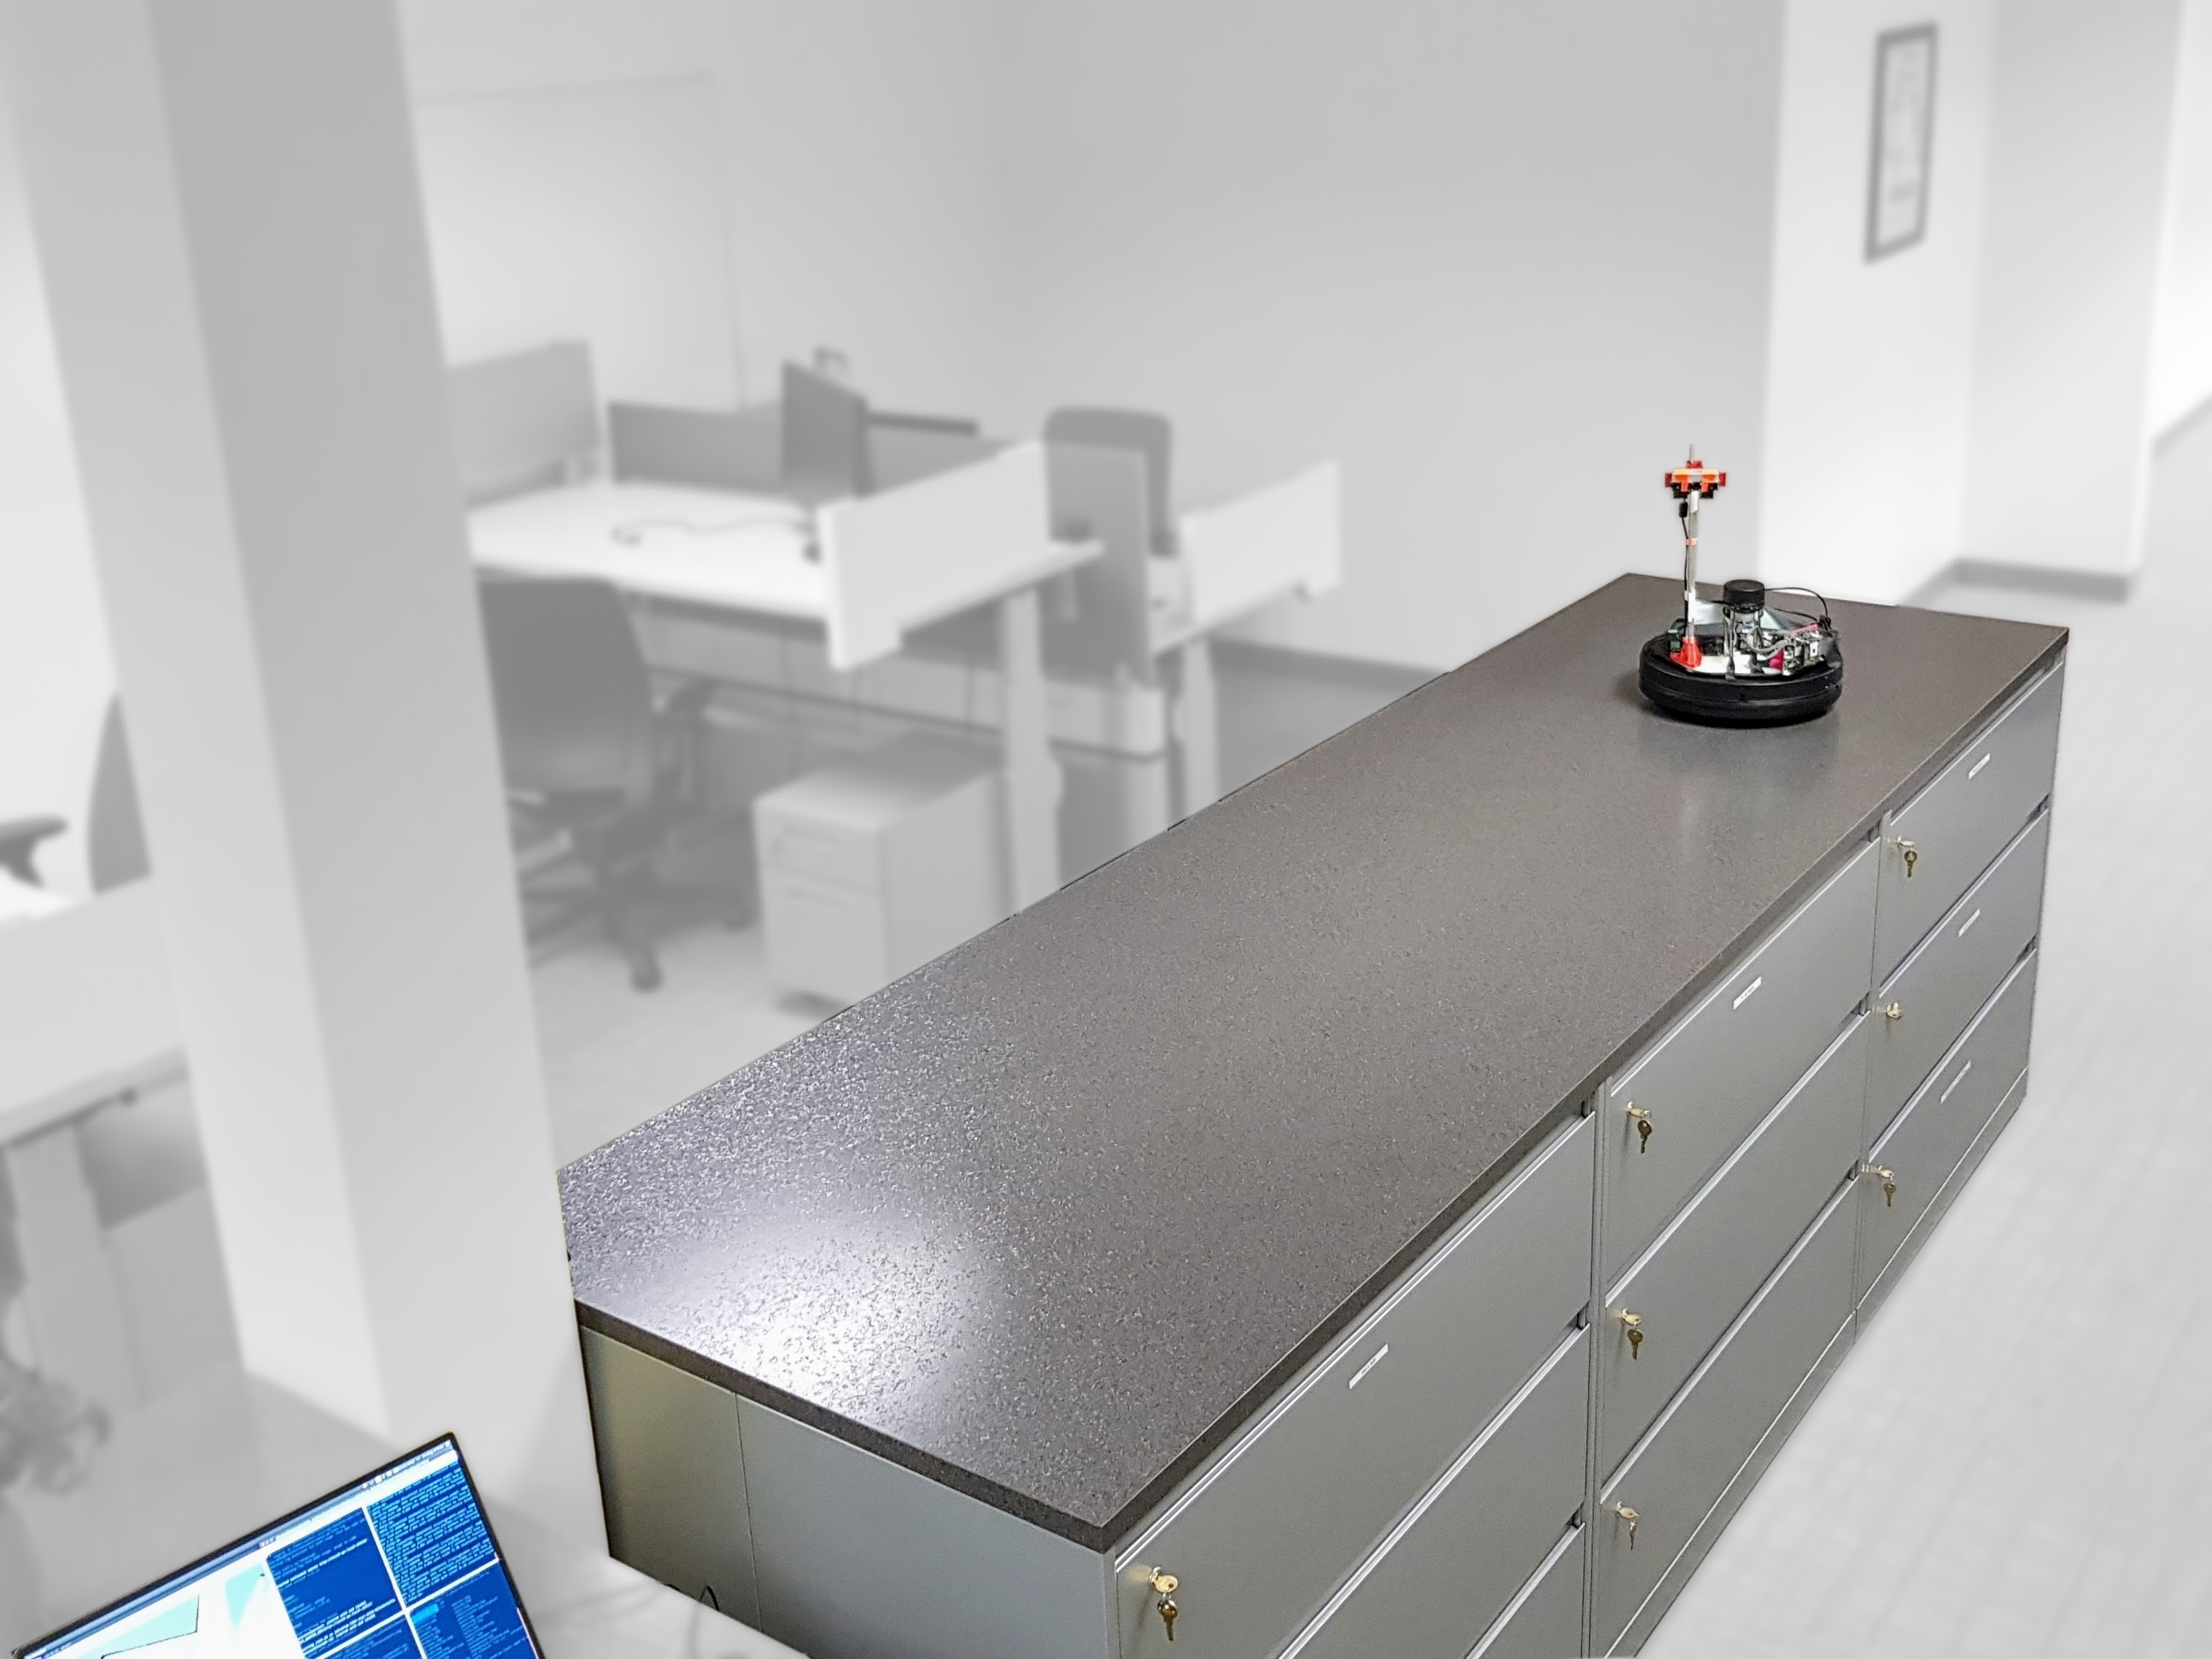
\includegraphics[width=\textwidth]{gfx/pictures/cliff}
        \caption{For the negative obstacle detection tests the robot was driving on the cabinet.}
        \label{fig:cliff}
    \end{subfigure}%
    \hfill%
    \begin{subfigure}[t]{.475\textwidth}
        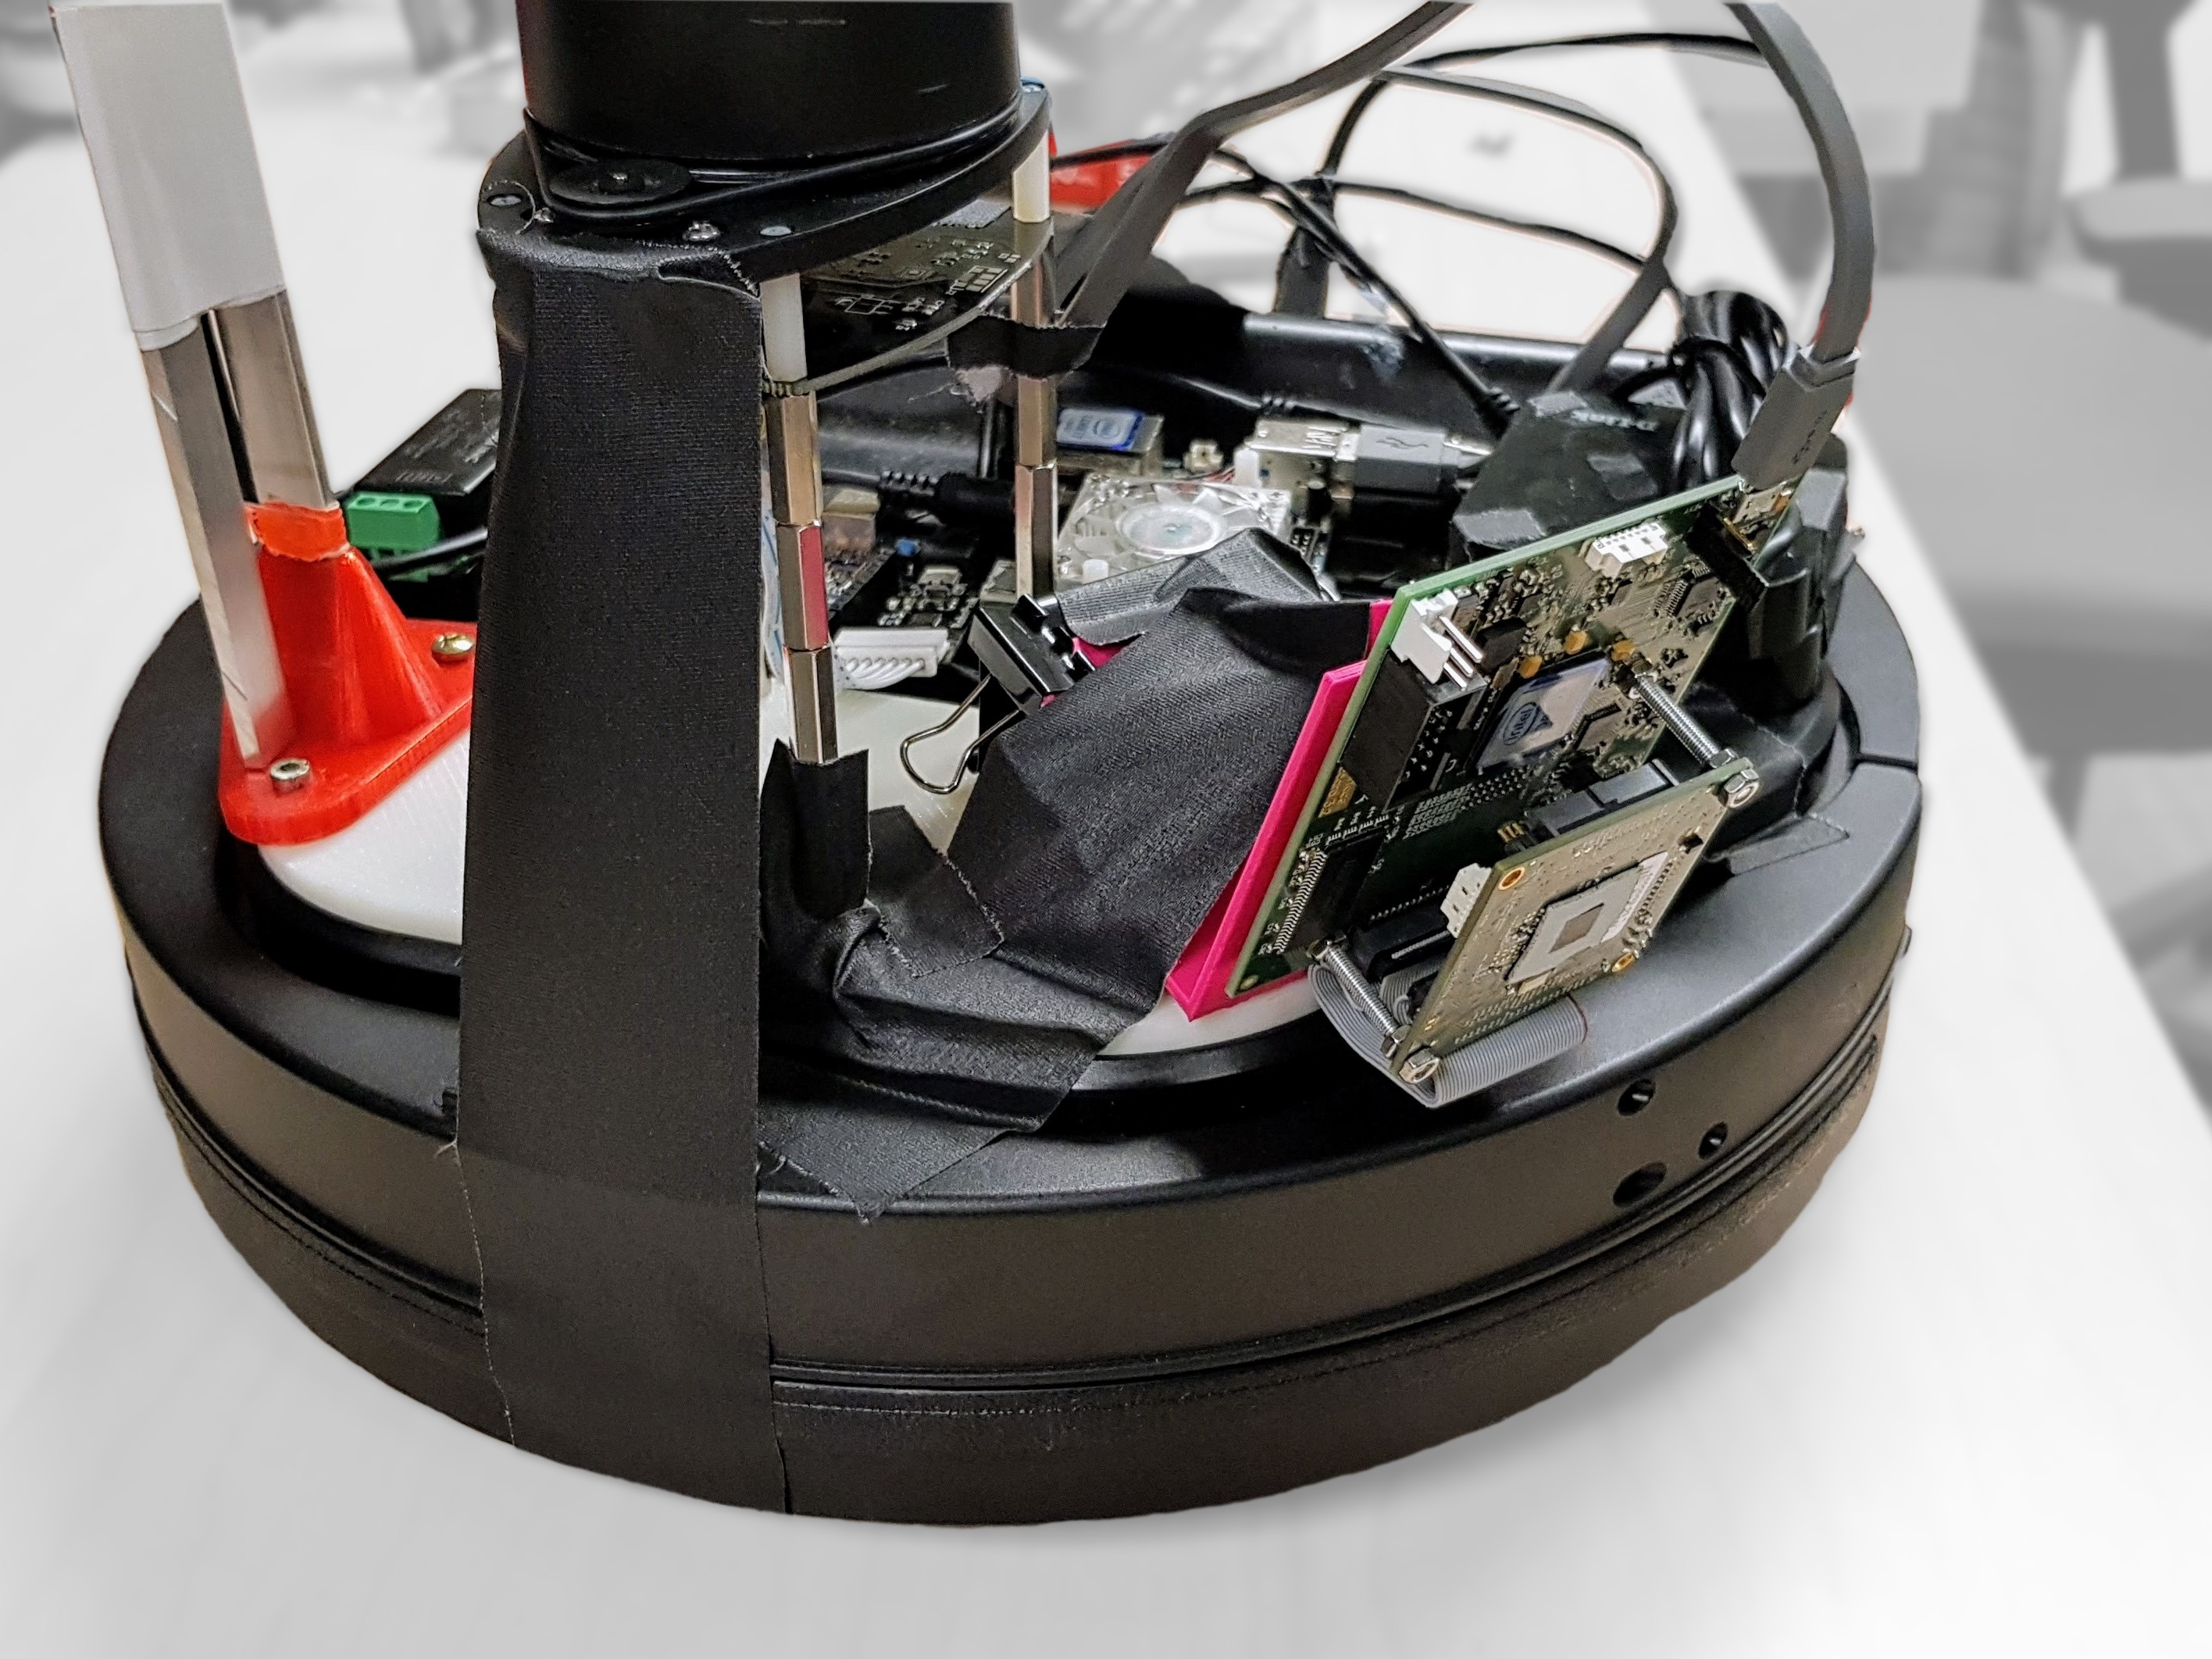
\includegraphics[width=\textwidth]{gfx/pictures/cliff_sensor}
        \caption{Sensor orientation for the Washroom scan: downward-facing vertical in an attempt to improve cliff detection}
        \label{fig:cliff_sensor}
    \end{subfigure}
\end{figure}

With scans V,W,X the negative obstacle detection capability was
analyzed in the environment shown in \cref{fig:cliff}. Cliffs, steps, and ditches are types of negative obstacles that cannot be traversed by the robot. In \cite{Jiang2015}, Jiang et al. claim that it is possible to detect this with UWB signals of various carrier frequencies. The experiments carried out for this thesis however did not show the same signal behaviour and it was not possible to reliably detect cliffs.

The Virtual Reality scan was carried out in the standard configuration
with a horizontal, slightly squinting, and not downwards angled sensor.
The assumption was that a part of the strong signal in the \SIrange{10}{20}{cm}
range was due to reflections from the floor, that should disappear when the
floor ends at a cliff. Visual inspection of the range profile however
shows only a extremely slight change in signal, e.g.~at cross range
\SIrange{0.8}{1.1}{m}, down range \SIrange{0.2}{0.25}{m}., where the floor could not reflect due to the radar sensor overhanging the cliff.

The Washroom scan has the sensor mounted in a vertical configuration and
downward facing (see \cref{fig:cliff_sensor}) instead to increase sensitivity to echo scattering from below. The echo intensity for cross range \SIrange{3.5}{4.5}{m} is indeed just
barely lower than \SIrange{0}{2}{m}, which matches up to where the sensor was over
the edge and over floor, respectively.

\begin{figure}[htbp]
    \centering
    \begin{subfigure}[t]{.475\textwidth}
        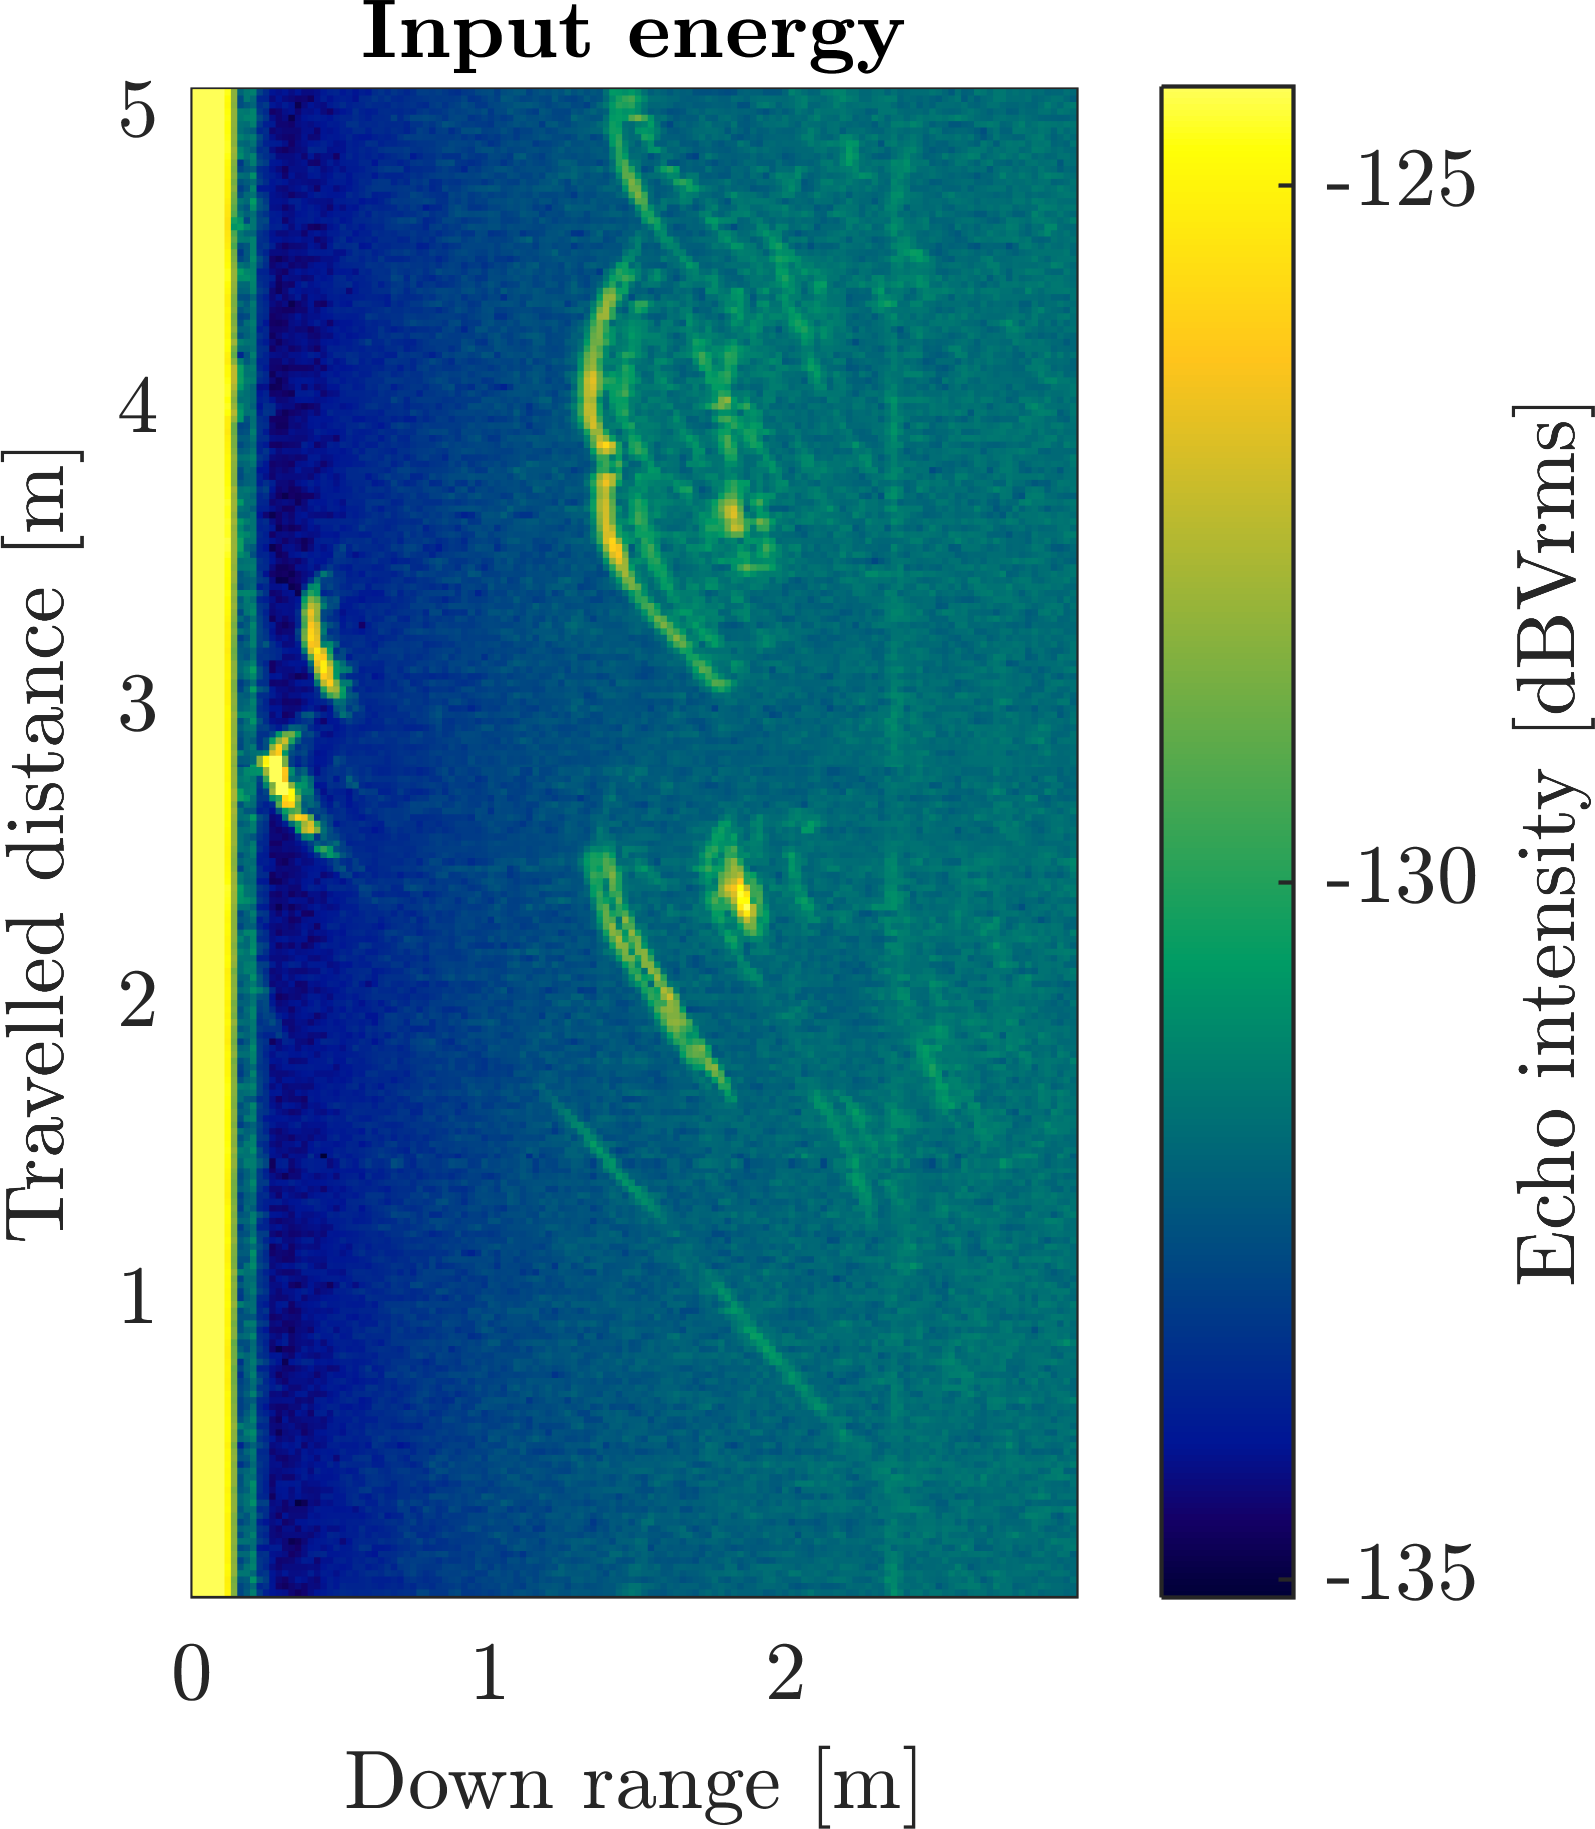
\includegraphics[max height=10cm,max width=10cm]{figures/fig_negobst}
        \caption{Regular plot.}
        \label{fig:negobst}
    \end{subfigure}%
    \hfill%
    \begin{subfigure}[t]{.475\textwidth}
        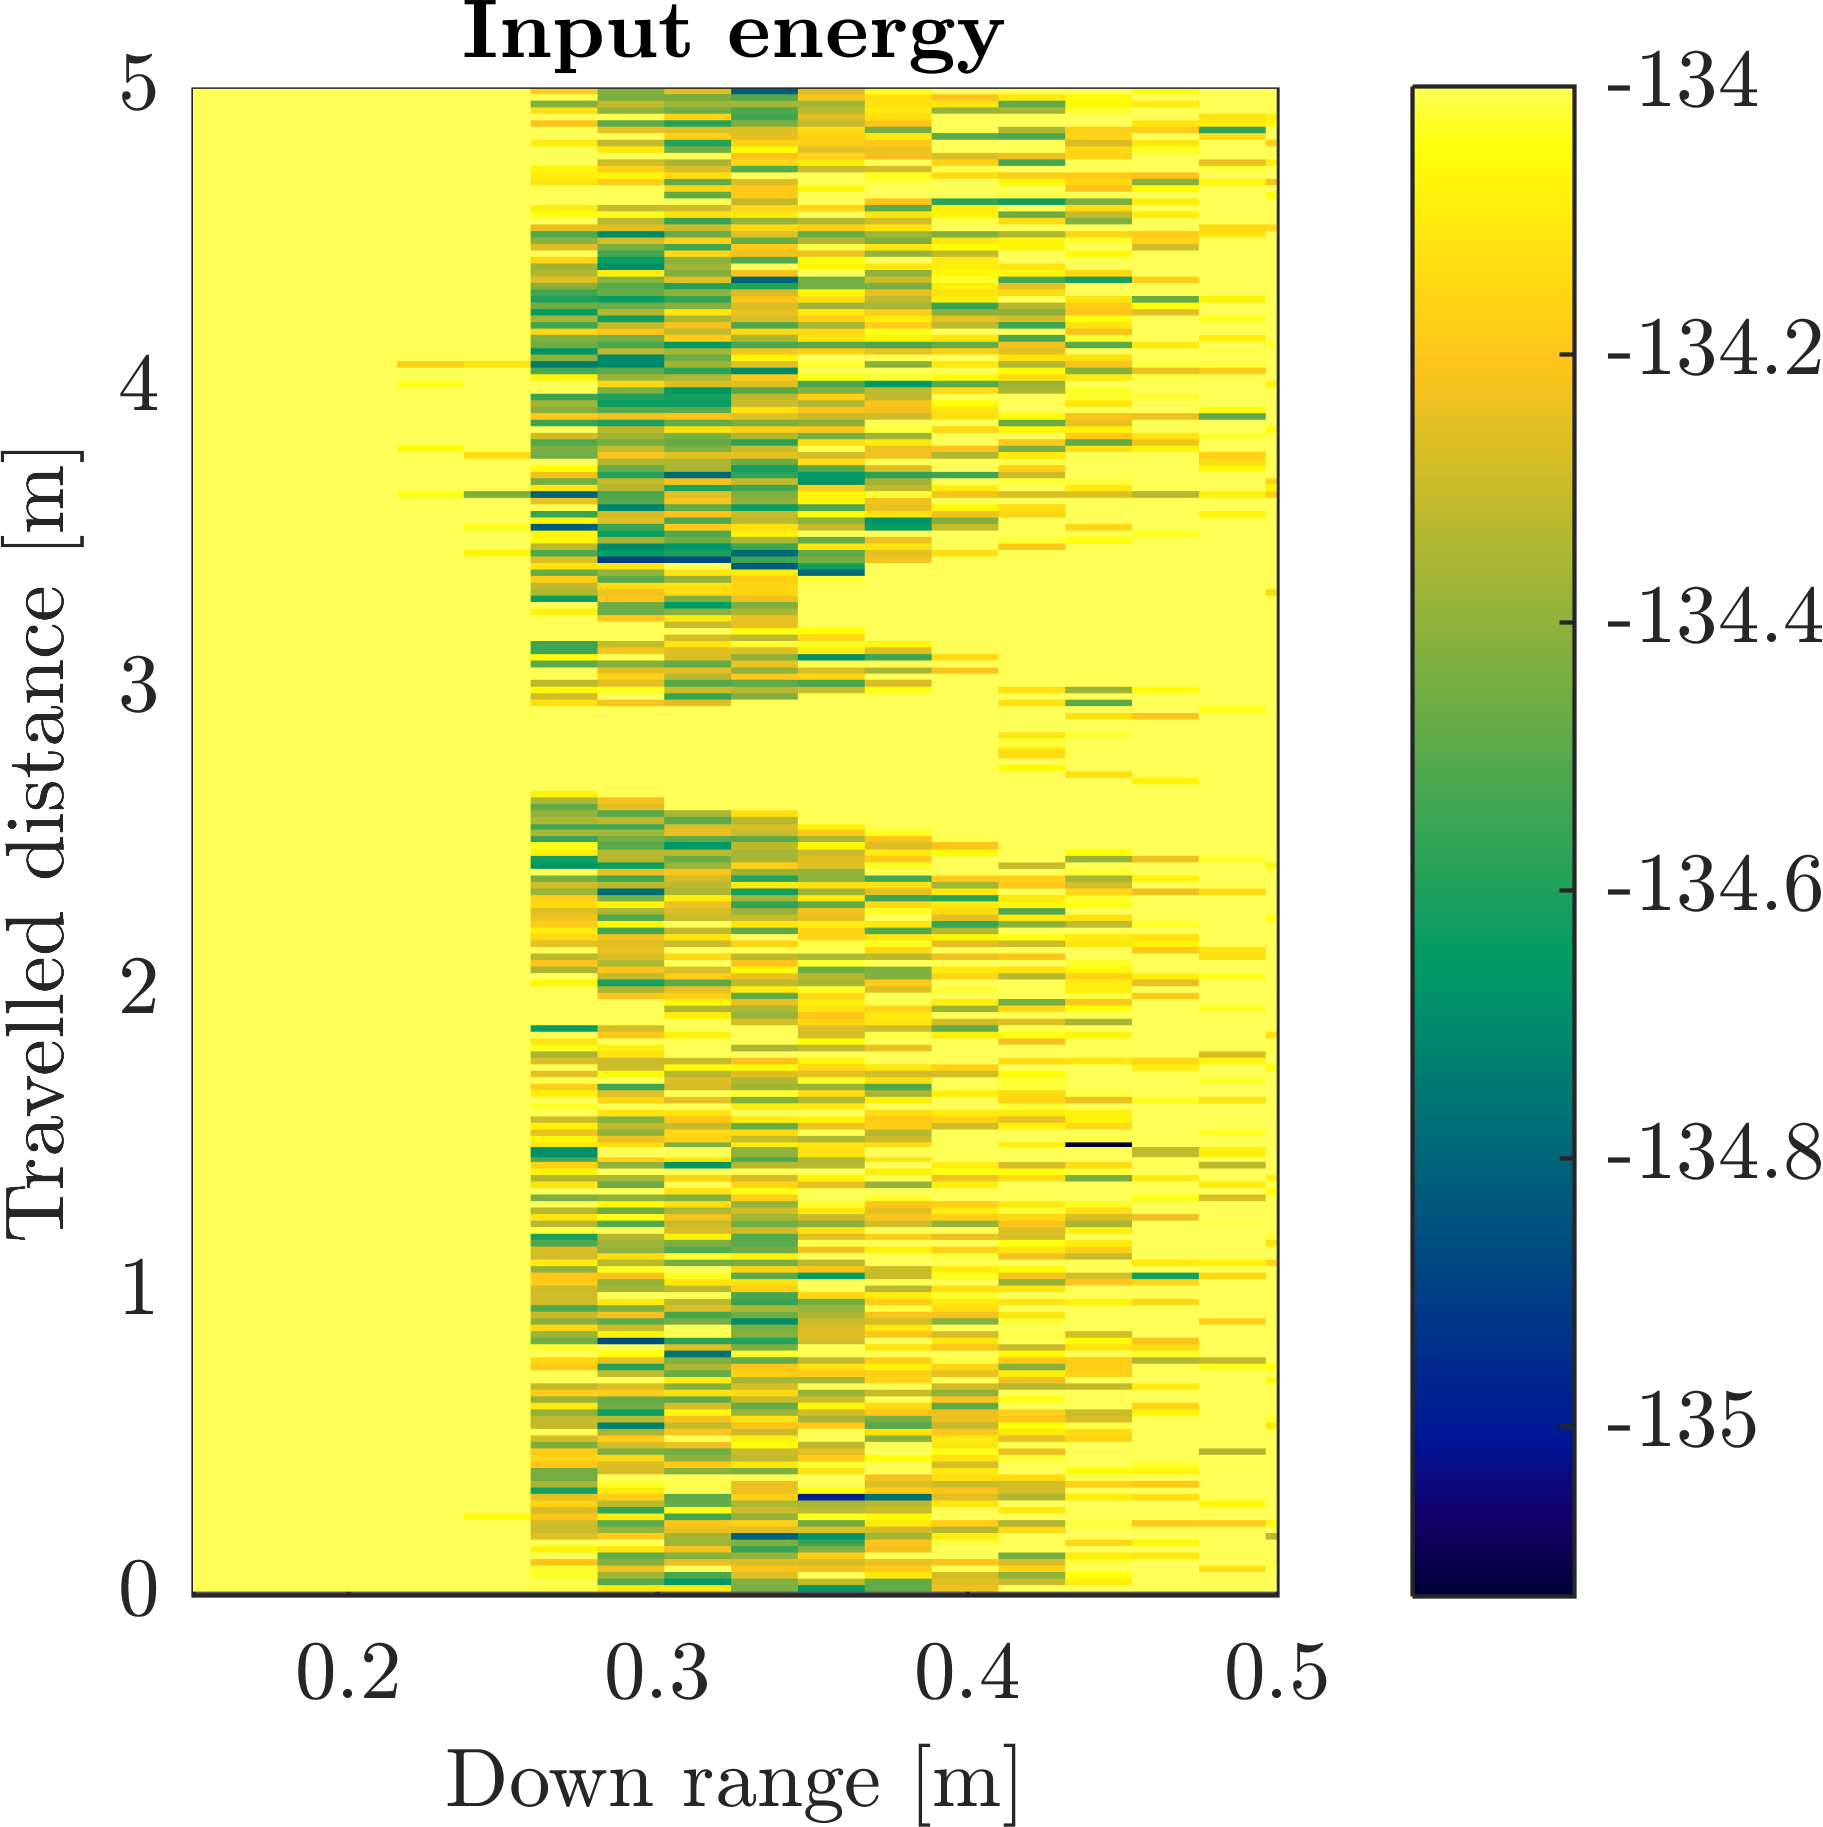
\includegraphics[max height=10cm,max width=10cm]{figures/fig_negobst_clipped}
        \caption{Zoomed and intensity-clipped for better visibility of the effect.}
        \label{fig:negobst_clipped}
    \end{subfigure}
    \caption{Input energy for the Washroom scan. Lower echo intensity at negative obstacles (annotated with arrow) is hardly visible in the standard configuration.}
\end{figure}

To limit the transmit crosstalk's blinding effect, the sensor was
mounted on a much higher position (on the RGBD camera mount) in the Xray
Room scan. One effect is that the robot chassis itself is constantly
visible at a distance of \SI{0.35}{cm} down range. At \SI{0.45}{cm} down range, the
floor echo is visible. There is one dip in intensity at \SI{2.5}{m} cross
range, where the sensor was not over floor. Overall the signal is
however not as conclusive as in the Washroom scan.

\begin{figure}[htbp]
    \centering
    \begin{subfigure}[t]{.475\textwidth}
        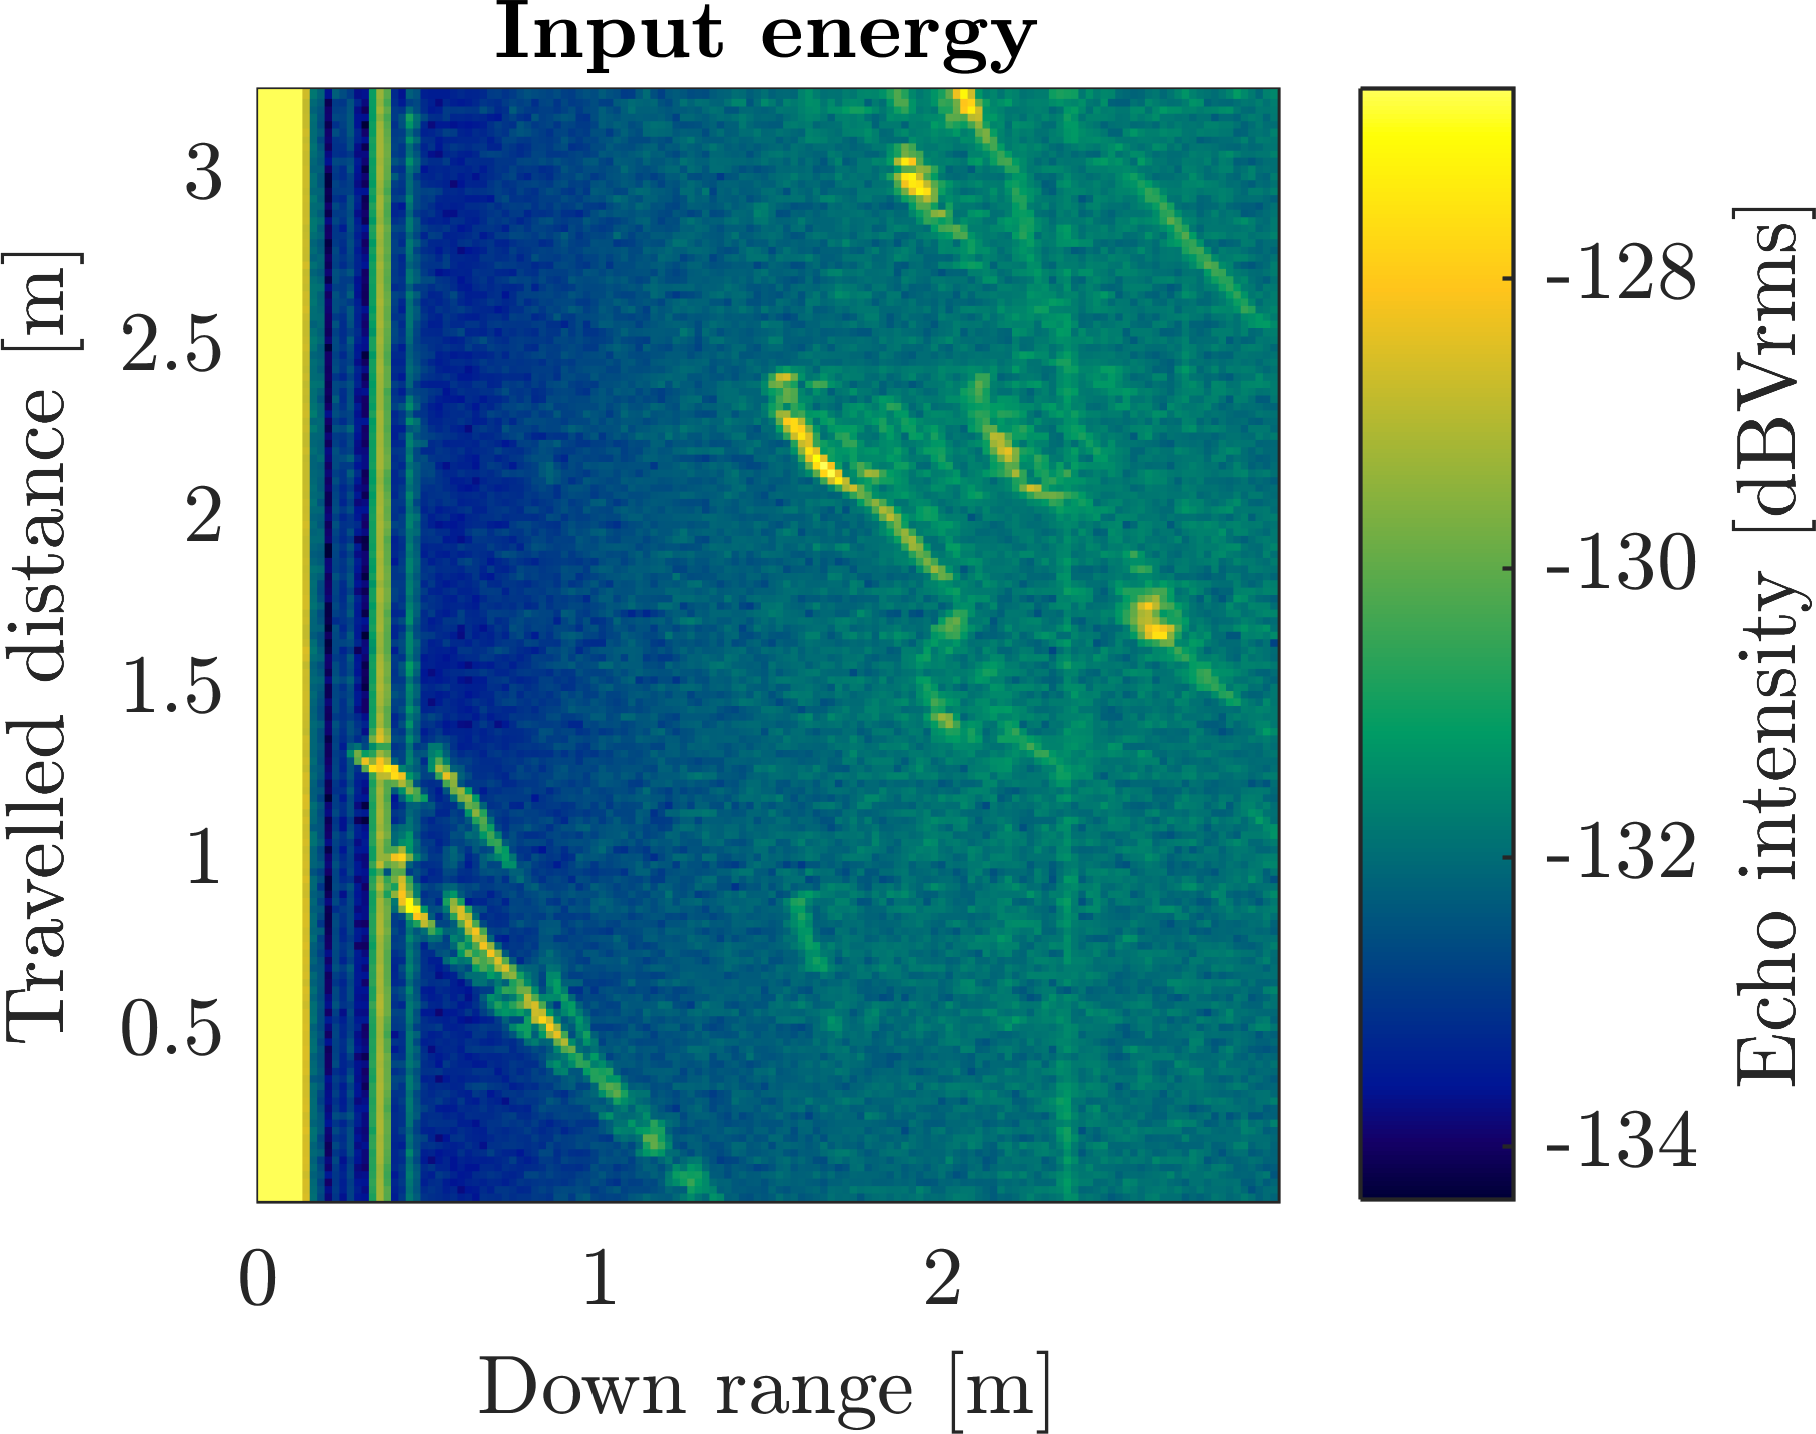
\includegraphics[max height=10cm,max width=10cm]{figures/fig_negobst_xray}
        \caption{Regular plot.}
        \label{fig:negobst_xray}
    \end{subfigure}%
    \hfill%
    \begin{subfigure}[t]{.475\textwidth}
        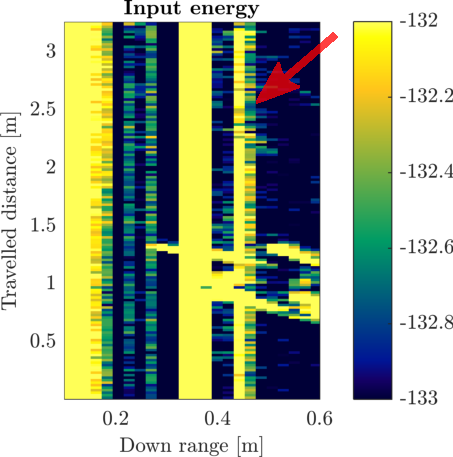
\includegraphics[max height=10cm,max width=10cm]{figures/fig_negobst_xray_clipped}
        \caption{Zoomed and intensity-clipped for better visibility of the effect.}
        \label{fig:negobst_xray_clipped}
    \end{subfigure}
    \caption{Input energy for the XRay Room scan. Negative obstacle effect is not better with a higher-mounted vertical configuration.}
\end{figure}


Maybe the signal could be improved with improved background subtraction, but the three scans show that it is generally very hard to
detect negative obstacles with this sensor. A radar sensor of this type
will hence not be a viable replacement for regular cliff detection
sensors like the floor facing infrared distance sensors in the Kobuki
base.

\subsection{Cable detection}\label{cable-detection}

Cables on the floor are another interesting target that falls into the
category of obstacles being a very common occurrence in the real world,
but are hard to detect with conventional obstacle sensors. The Y (Is
There A Cable On The Floor) scan deals with the detection if this kind
of obstacle. For this, the same camera-mounted vertical configuration as
in X Ray Room was used. Again, there is a constant robot chassis echo at
down range \SI{0.35}{m}. As the robot is driving closer towards the power cable
on the floor, the cable's echo is visibly coming closer before it
disappears under the robot's chassis. The echos at \SI{0.9}{m} down range show
the two can towers at the end of the cable.

\begin{figure}[htp]
    \centering
    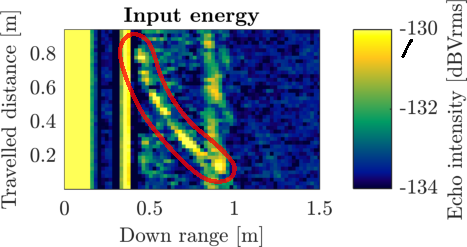
\includegraphics[max height=10cm,max width=10cm]{figures/fig_cable}
    \caption{Input energy of the Y (Is There A Cable On The Ground) scan. The arc (circled in red) represents the echo of a cable on the floor as the robot approaches.}
    \label{fig:cable}
\end{figure}

Both the X Ray Room and Y (Is There A Cable On The Floor) introduce a
new geometry that lifts the radar sensor out of the two dimensional
mapping plane. The geometry is better described with the 3D case in \cref{geometry-for-the-3d-case}.

The results suggest that cables can be detected, but it might be hard to decide if the robot can safely drive over them.

\subsection{Minimum distance}\label{minimum-distance}

The constant noise from the transmission crosstalk leads to a high
minimum detection distance as explained in \cref{transmit-crosstalk-suppression}. The effect is that
targets can not be projected onto the map if the robot is too close to
them. This is an issue in the Sauna scan, where the glass wall right at
the beginning of the robot path cannot be mapped easily without introducing some phantom targets caused by the transmission crosstalk.

\subsection{Noise} \label{noise}
As stated in \cref{optimal-chirp-time-configuration}, the signal and noise levels in the input energy are influenced strongly by a scan's sweep duration. This can be observed when comparing the input energy plots of the P,Q,R,S scans (see \cref{fig:res_p,fig:res_q,fig:res_r,fig:res_s}), whose scan parameters vary only in sweep duration (5, 20, 2, and \SI{2.5}{ms}, respectively). The \SI{20}{ms} scan in \cref{fig:res_q} features very high noise in some cross-range areas. This comes from broken and glitched radar packages which get smoothed out. Without these glitches, many targets would have intense echos, which facilitates mapping them. In future versions, either a glitch detection should be implemented to avoid this kind of noise, or the radar firmware/driver communication should be corrected to prevent glitches in the first place. The \SI{5}{ms} scan in \cref{fig:res_p} still has the occasional broken packet, but is overall much cleaner, which a good SNR. The \SI{2.5}{ms} scan in \cref{fig:res_s} is comparable to the \SI{2.0}{ms} scan in \cref{fig:res_r} and both still have a good SNR. As concluded in \cref{optimal-chirp-time-configuration}. \SI{5}{ms} are a good compromise between good SNR from the long sweep time and a low probability of glitches occuring.

The \SI{2.5}{ms} scan has another kind of noise in it: there is a constantly visible peak at around \SI{1}{m}, corresponding to a range frequency of ca. \SI{24}{kHz}. The harmonics of this frequency are also visible at \SI{2}{m} and so on. The constant frequency suggests that some onboard electronics introduce this noise. \cite{Ernst2016} observed some SPI bus noise on the original board, and this could be related. It is however easy to work around by erasing the offending input data: \texttt{range(:,down\_range>0.98 \& down\_range<1.07) = nan;}. The harmonics are below the minimum peak threshold, so they do not cause harm. Another easy way of getting around this issue is to choose a sweep time other than \SI{2.0}{ms}.

In the close down range (<\SI{0.5}{m}), there are two kinds of noise sources: One is the transmit crosstalk explained in \cref{transmit-crosstalk-suppression} and the other one is ground echo. Ground echo only plays a role in vertical beam fan shape configuration (``V'' in \cref{tab:params}); horizontal beam fan orientations have sufficient elevation focus to be unaffected. Scans D-I have therefore a slightly higher noise level right after the transmit crosstalk noise.

The signal level is also further boosted with the plastic horn antenna extension, at the cost of seeing targets only in a limited field of view and hence for a shorter amount of time. The reprojection maps have similar quality. With the horn extension installed, targets that are farther away are detected more reliably. In a mostly side-facing geometry, targets that lie more ahead of the robot than off to the side of the motion path are detected earlier with the horn extension removed. So applications like obstacle avoidance, where early detection is important should use a wider beam (i.e. no horn extension) and applications geared towards mapping even at range should use a more narrow beam (i.e. horn extension installed).



%%%%%%%%%%%%%%%%%%%%%%%%%%%%%%%%%%%%%%%%%%%%%%%%%%%%%
\section{Comparison with other mapping techniques} \label{comparison-with-other-mapping-techniques}

While some of the radar reprojection maps speak for themselves, they
make more sense when compared to other mapping techniques. In the
following, SAR techniques, Laser slam, and RGBD slam are compared to the
radar reprojection.

\subsection{SAR}\label{sar-1}
Synthetic aperture radars make a lot of sense in applications
where the radar is moved over or through a map. The big difference to
this application is that ``professional'' SAR applications have radar
sensors that sit in vehicles that are not in the mapping plane.
Airplanes, satellites and even Submarines scan the earth like that.

There are a few examples for UWB radars being moved sideways (usually on a rail) in an effort to scan a scene with synthetic aperture radar.
Gregory L. Charvat's ``tin can'' radar \cite{Charvat2014} might be the most famous one, with many examples at \url{http://glcharvat.com/shortrange/}.
Another great resource was Henrik Forstén's Homemade Synthetic Aperture
Radar, documented in \cite{Forsten2015} (see \cref{fig:forsten}). He used an Omega-k algorithm \cite{Tolman2008} and Stolt interpolation \cite{Cumming2004} to correct the range migration arcs.

\begin{figure}[htbp]
% 0.95 * 3264*817/2448 / (3264*817/2448 + 1299) = 0.43330076762
% 0.95 * 1299 / (3264*817/2448 + 1299) = 0.51669923238
    \begin{subfigure}[t]{0.43330076762\textwidth}
        \centering
        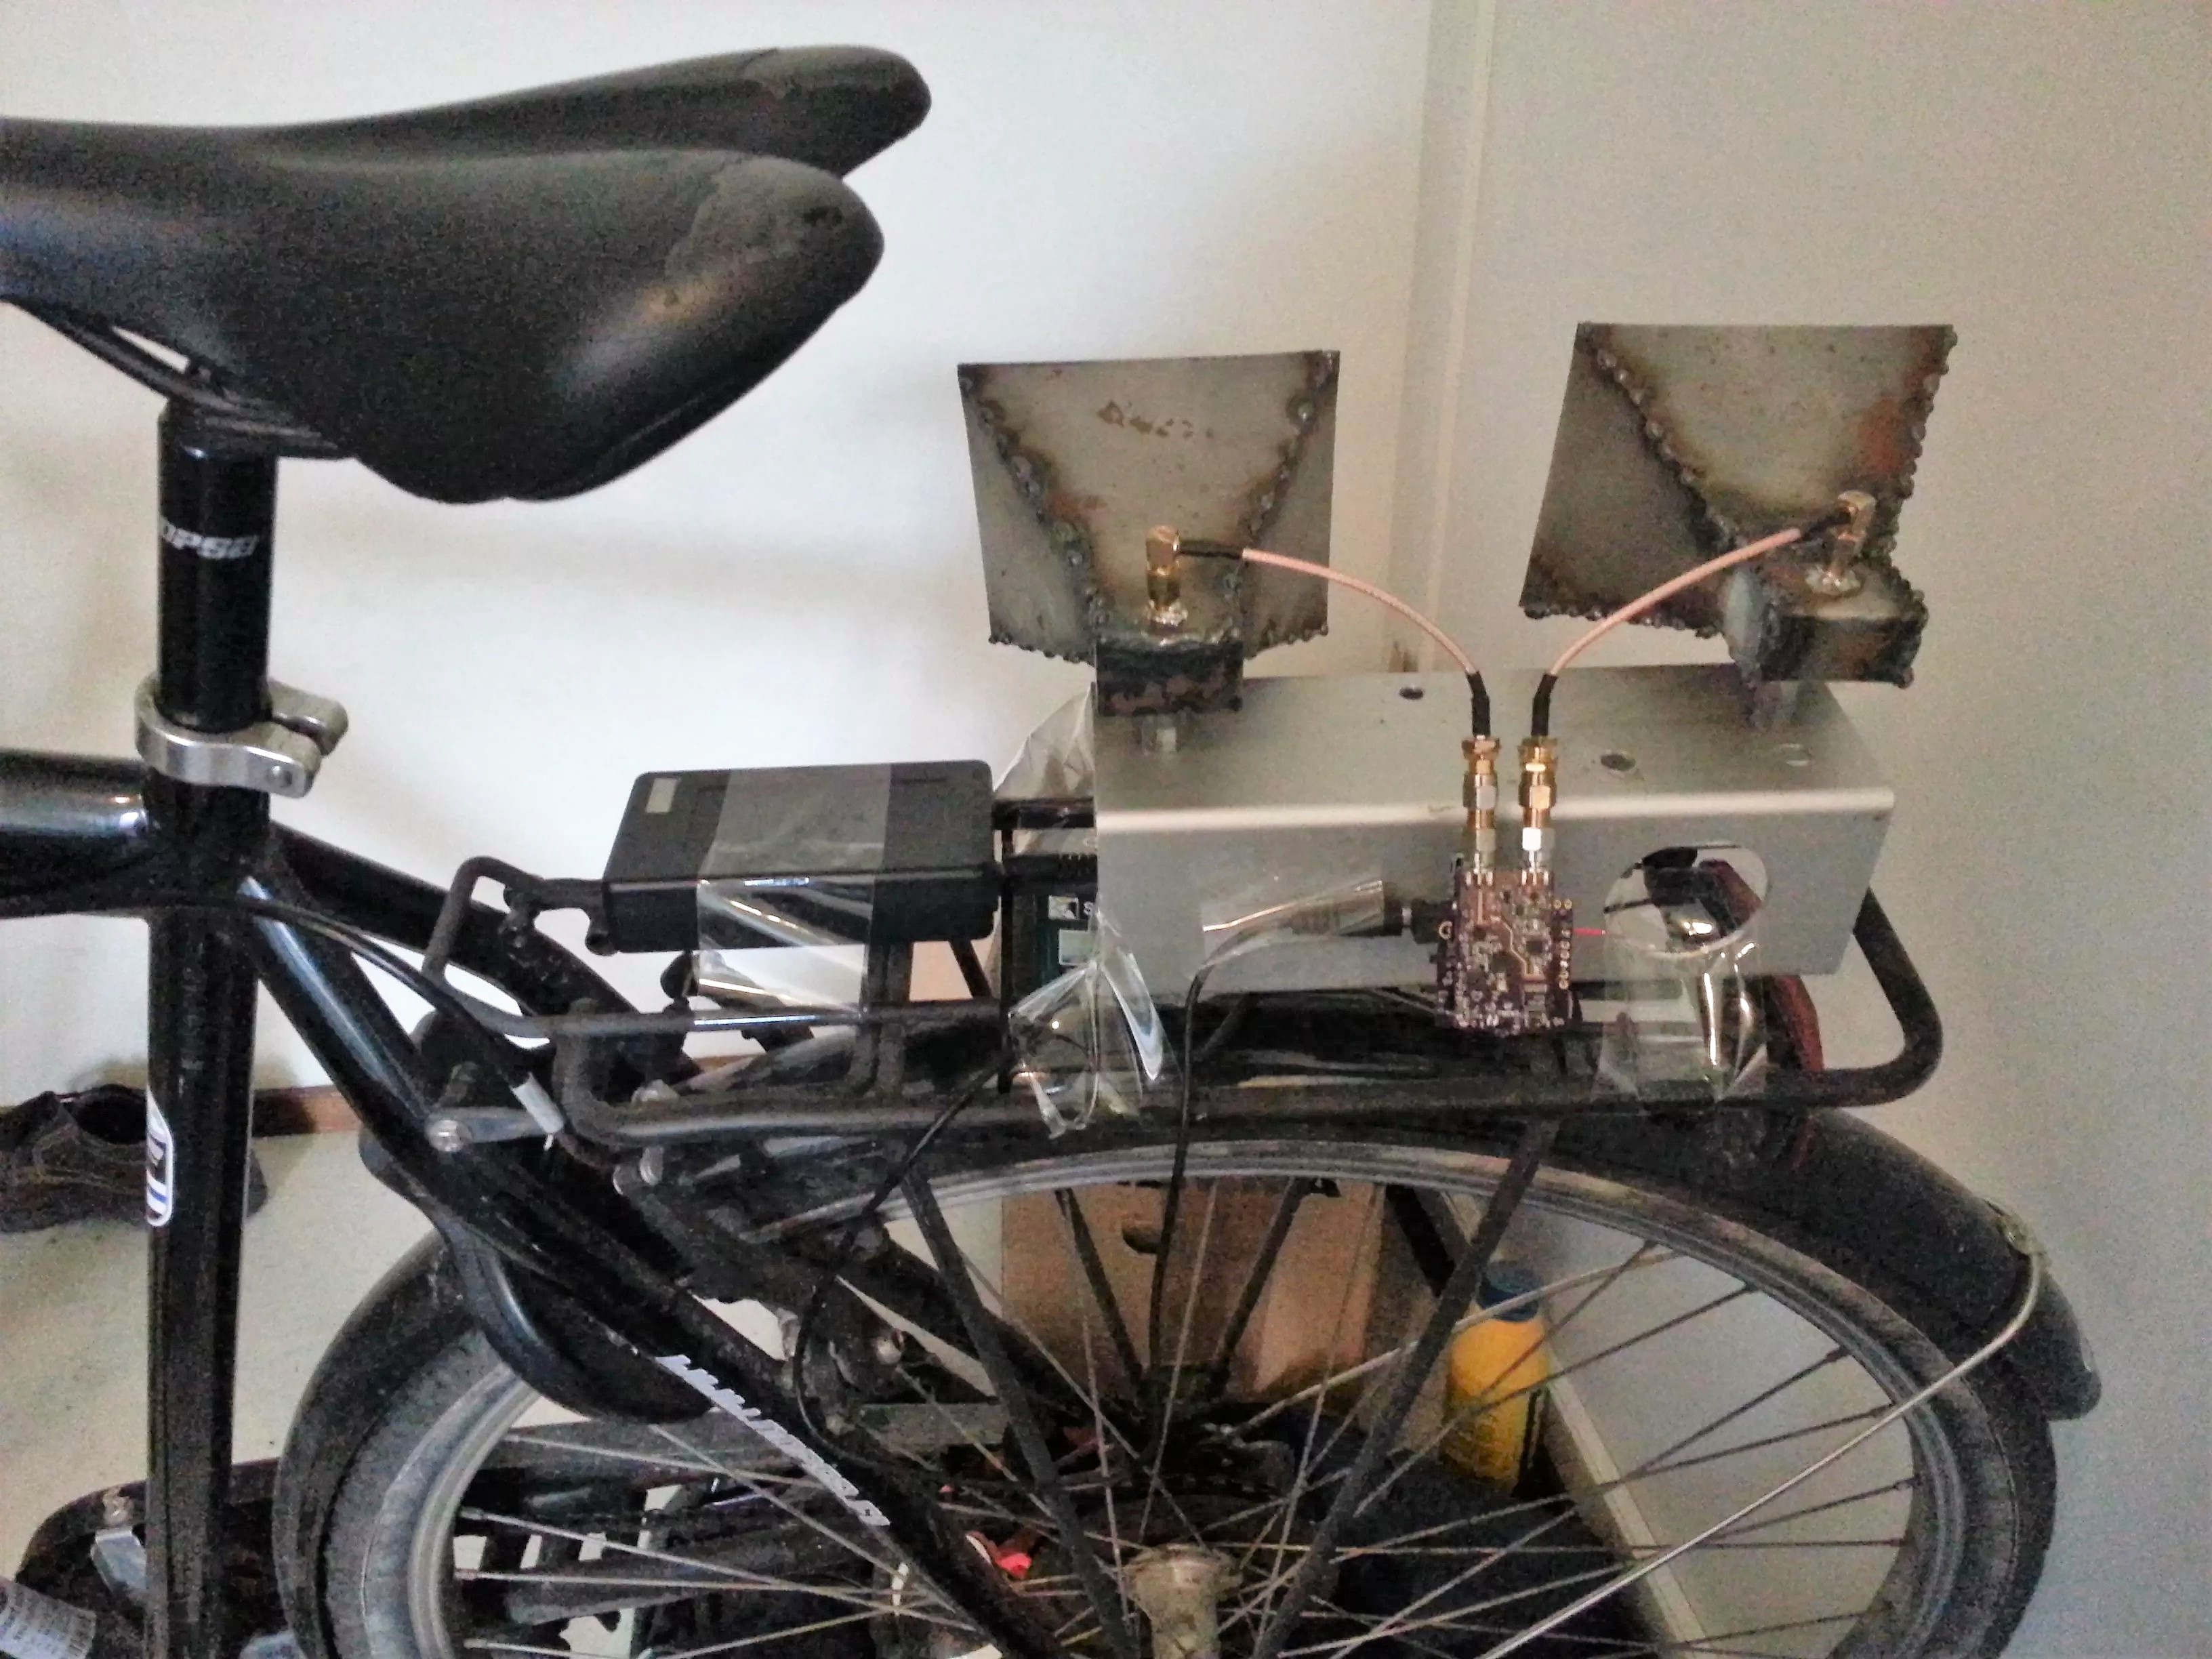
\includegraphics[max width=\linewidth]{gfx/pictures/forsten_1.jpg}
        \caption{Forstén's SAR setup. Source: \cite{Forsten2015}}
        \label{fig:forsten_1}
    \end{subfigure}%
    \hfill%
    \begin{subfigure}[t]{0.51669923238\textwidth}
        \centering
        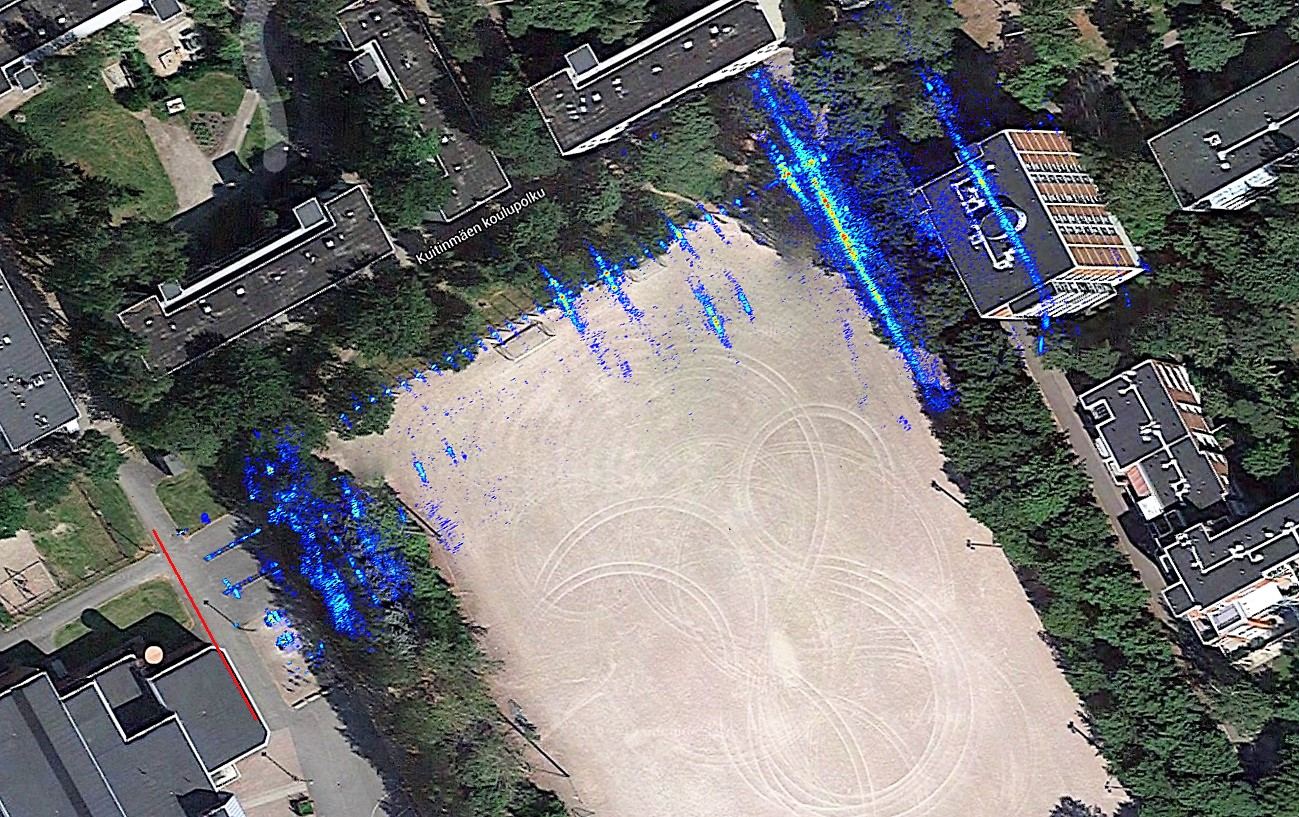
\includegraphics[max width=\linewidth]{gfx/pictures/forsten_2.jpg}
        \caption{Forstén's SAR imagery agrees well with aerial imagery. Source: \cite{Forsten2015}}
        \label{fig:forsten_2}
    \end{subfigure}
    \caption{After omega-k processing and autofocusing, Forstén's synthetic aperture radar can create nice-looking broadside SAR imagery.}
    \label{fig:forsten}
\end{figure}

Forstén was able to greatly improve his data quality by use of a minimum-entropy based auto-focusing algorithm. The trick with this is that the radar needs to move in a very straight line, where the ``error in path linearity should be around less than tenth of a wavelength'' \cite{Forsten2015}. In Forstén's radar, this is about \SI{5}{mm}. However with the \SI{60}{GHz} Omniradar this is around \SI{0.5}{mm}. Keeping a straight line with less than half a millimeter of linearity error is not realistically achievable on the Kobuki platform.


One big inherent problem with synthetic aperture radar algorithms is
that basically all of them assume the radar to move in a straight line.
While changing the squint angle helps to deal with issues such as earth
curvature in satellite applications, SAR with curved or even arbitrary
paths is a challenging topic, particularly because auto-focusing, which
again relies on phase information, becomes more difficult
\cite{Axelsson2002}.

In \cite{Watts2016}, Watts, \textit{et al.} showed experiments with conceiled SAR imaging on a PR2 robot (see \cref{fig:pr2}). Their radar sensor had \SI{11.5}{GHz} of bandwidth available and is able to create SAR imagery with high precision. However, they relied on classic SAR geometry and moved the radar sensor in a straight line.

\begin{figure}[htbp]
    \centering
    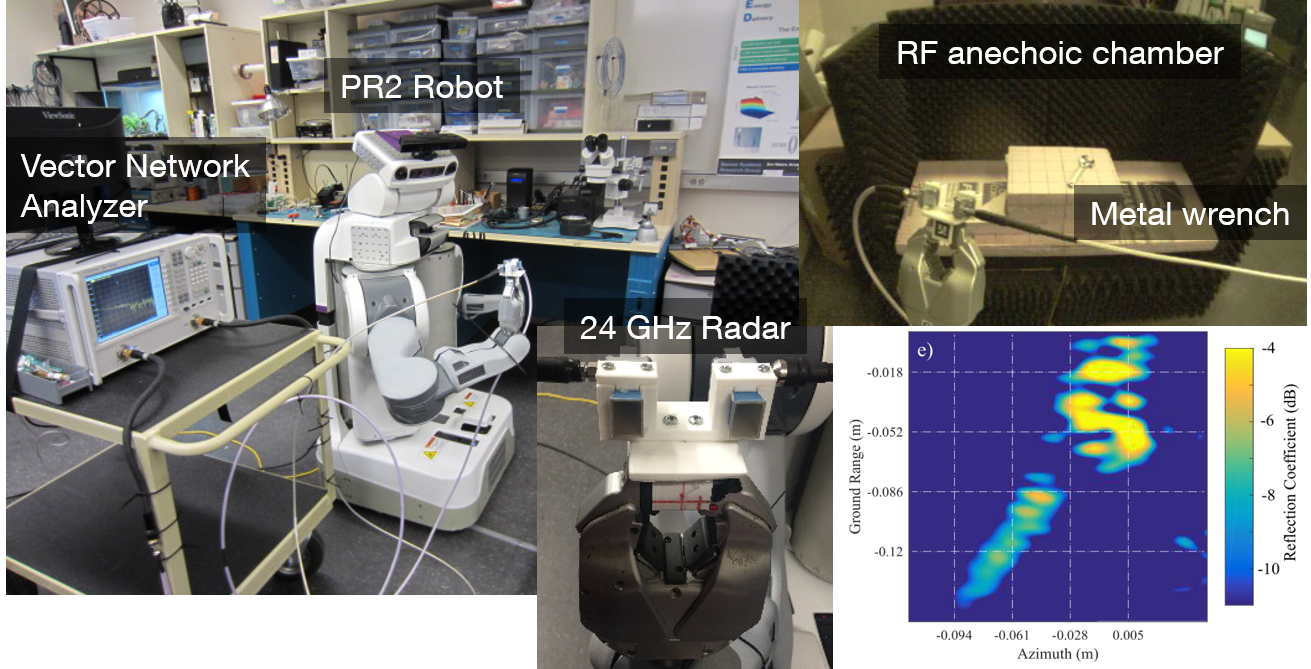
\includegraphics[max width=\textwidth]{gfx/pictures/pr2_sar.png}
    \caption{A PR2 robot performing conceiled SAR imaging by moving the radar sensor attached to its gripper in a straight line. Source: \cite{Watts2016}.}
    \label{fig:pr2}
\end{figure}


\subsection{RGBD}\label{rgbd-1}
The Kobuki robot was also carrying an Astra Orbbec Mini\footnote{\url{https://orbbec3d.com/astra-mini/}} strutured light depth camera. Using the Rtabmap \cite{Labbe2014} ROS package\footnote{\url{http://wiki.ros.org/rtabmap_ros}}, some 3D scans of the office environment where made. \cref{traditional-obstacle-sensors} already showed the shortcomings of lidar and RGBD sensors, but in this section the same \cref{fig:lidar_rgbd2,fig:rgbd_glasswall2} are compared with radar reprojection.

\Cref{fig:chairlegs} shows clearly that the radar reprojection contains horizontal chair legs, while the lidar scan does not. The scene in \cref{fig:rgbd_glasswall2} matches with the Underground scan, where the glass wall is clearly visible.

\begin{figure}
    \begin{subfigure}[t]{.485\textwidth}
        \centering
        \includegraphics[max width=\textwidth]{gfx/pictures/torturechamber_scene}
        \caption{View of the Torturechamber scan environment. Blue path is the robot's path.}
        \label{fig:chairs_scene}
    \end{subfigure}%
    \hfill%
    \begin{subfigure}[t]{.485\textwidth}
        \centering
        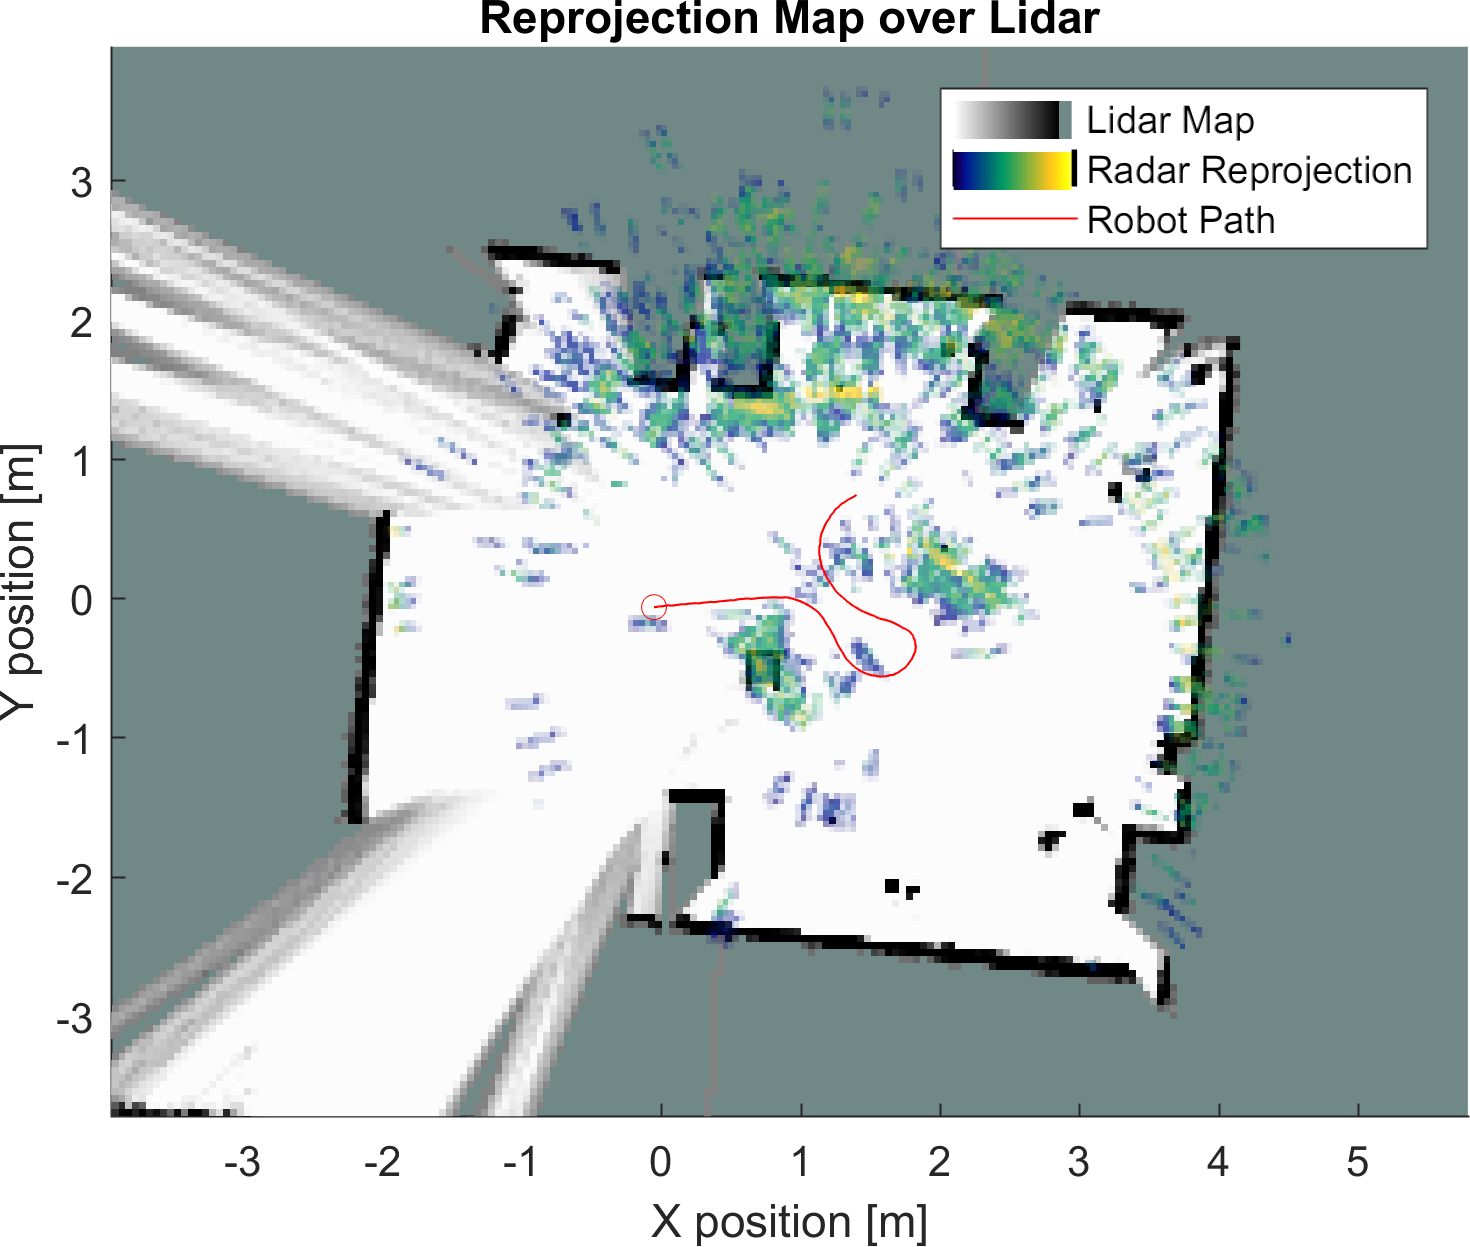
\includegraphics[max width=\textwidth]{gfx/results/torturechamber_map}
        \caption{Torturechamber reprojection map over lidar slam gridmap.}
        \label{fig:chairs_map}
    \end{subfigure}%
    \caption{In the Torturechamber scan, horizontal chair legs are visible in the reprojection map but not in the lidar scan.}
    \label{fig:chairlegs}
\end{figure}

\subsection{Lidar}\label{lidar-1}
As stated in \cref{kobuki}, the Kobuki robot used in the experiments was equipped with an RPLidar and a computing platform powerful enough to perform slam. Lidar slam is the standard approach when it comes to mapping the environment around a robot. After years of research and product development, even relatively cheap lidar systems like the RPLidar have acceptable range resolution. While they can't provide ground truth data (see problems with lidar data in \cref{traditional-obstacle-sensors}), it makes sense to compare the radar reprojection maps with laser scan maps. This is why all scans after Mancave have lidar maps associated.
%TODO?
Note that there is a bug in the rosbag to Matlab conversion that sometimes causes the complete map to be rotated against the lidar map by some degrees.
